%%%%%%%%%%%%%%%%%%%%%%%%%%%%%%%%%%%%%%%%%%%%%%%%%%%%%%%%%%%%%%%%%%
%%%%%%%% ICML 2016 EXAMPLE LATEX SUBMISSION FILE %%%%%%%%%%%%%%%%%
%%%%%%%%%%%%%%%%%%%%%%%%%%%%%%%%%%%%%%%%%%%%%%%%%%%%%%%%%%%%%%%%%%

% Use the following line _only_ if you're still using LaTeX 2.09.
%\documentstyle[icml2015,epsf,natbib]{article}
% If you rely on Latex2e packages, like most moden people use this:
\documentclass{article}

% use Times
\usepackage{times}
% For figures
\usepackage{graphicx} % more modern
%\usepackage{epsfig} % less modern
\usepackage{subfigure} 

% For citations
\usepackage{natbib}

% For algorithms
\usepackage{algorithm}
\usepackage{algorithmic}

% As of 2011, we use the hyperref package to produce hyperlinks in the
% resulting PDF.  If this breaks your system, please commend out the
% following usepackage line and replace \usepackage{icml2016} with
% \usepackage[nohyperref]{icml2016} above.
\usepackage{hyperref}
\hypersetup{
	colorlinks   = true, %Colours links instead of ugly boxes
	urlcolor     = blue, %Colour for external hyperlinks
	linkcolor    = blue, %Colour of internal links
	citecolor   = blue %Colour of citations
}

% Packages hyperref and algorithmic misbehave sometimes.  We can fix
% this with the following command.
\newcommand{\theHalgorithm}{\arabic{algorithm}}

% my settings
\usepackage{amsmath}\allowdisplaybreaks
\usepackage{amssymb,amsfonts,bbm}
\usepackage{mathrsfs}
\usepackage[all]{xy}
\usepackage{empheq}
\usepackage{algorithm,algorithmic}
\usepackage{multirow}
\usepackage{ifthen}
\usepackage[usenames]{color}
\usepackage[usenames,dvipsnames]{xcolor}
\usepackage{epstopdf}
%\usepackage{epsfig}
%\usepackage{times}
%\usepackage{helvet}
%\usepackage{courier}
%\usepackage{graphicx,subfigure}
%\usepackage{pdfpages}
%\usepackage{multirow}
%\usepackage{multicol}
\newcommand{\bbeta}{\boldsymbol{\beta}}
\newcommand{\EE}{\mathbb{E}}
\newcommand{\II}{\mathbb{I}}
\newcommand{\PP}{\mathbb{P}}
\newcommand{\RR}{\mathbb{R}}
\newcommand{\bT}{\mathbb{T}}
\newcommand{\bOne}{\mathbbm{1}}
\newcommand{\bA}{\mathbf{A}}
\newcommand{\ba}{\mathbf{a}}
\newcommand{\bB}{\mathbf{B}}
\newcommand{\bO}{\mathbf{O}}
\newcommand{\br}{\mathbf{r}}
\newcommand{\bU}{\mathbf{U}}
\newcommand{\bV}{\mathbf{V}}
\newcommand{\bw}{\mathbf{w}}
\newcommand{\bX}{\mathbf{X}}
\newcommand{\bY}{\mathbf{Y}}
\newcommand{\cA}{\mathcal{A}}
\newcommand{\cB}{\mathcal{B}}
\newcommand{\cH}{\mathcal{H}}
\newcommand{\cO}{\mathcal{O}}
\newcommand{\cS}{\mathcal{S}}
\newcommand{\argmax}{\mathrm{argmax}}
\newcommand{\trace}{\mathrm{trace}}
\newcommand{\abs}[1]{\left| #1 \right|}
\newcommand{\norm}[1]{\| #1 \|}
\newtheorem{theorem}{Theorem}[section]
\newtheorem{remark}[theorem]{Remark}
\newtheorem{proposition}[theorem]{Proposition}%[chapter]
\newtheorem{definition}[theorem]{Definition}%[chapter]
\newtheorem{corollary}[theorem]{Corollary}%[chapter]
\newtheorem{lemma}[theorem]{Lemma}%[chapter]
\newtheorem{example}[theorem]{Example}
\newenvironment{proof}{\noindent {\textbf{Proof. }}}{$\Box$ \medskip}

\newcommand{\CLemmaPrefixExi}{
	Suppose $1 = \gamma_1 \geq \gamma_2 \geq \cdots \geq \gamma_K \geq 0$. Let $A = (a_1, ..., a_{\abs{A}})$. For the time $t$ and the conjunctive objective, there exists a prefix $B$ of $A$ such that 
	$$
	p_{t, B} \geq \frac{\alpha}{2}f_{t}^{\ast} - 1 + \gamma_{\abs{B}}, \qquad R^{\alpha}(t, B) \geq \frac{1}{2} R^{\alpha}(t, A).
	$$ 
}
\newcommand{\CEqDeltaEstAnd}{
	$$
	\EE [R^{\alpha}(t, \bA_t) |\cH_t ] \leq \frac{8}{\alpha f^{\ast}} \EE \left[ \left. \bbeta_{t-1}(\delta)\sum_{k=1}^{\bO_t}\norm{\gamma_k x_{t,\ba_k^t}}_{\bV_{t-1}^{-1}} \right| \cH_t\right].
	$$
}
\newcommand{\CLemmaSumXiEstimateInDet}{
  If $\lambda \geq C_\gamma$, then
  $$
    \sum_{s=1}^t \sum_{k=1}^{\bO_s} \norm{\gamma_k x_{s,\ba_{k}^s}}_{\bV_{s-1}^{-1}}^2 \leq 2\ln \left(\frac{\det(\bV_t)}{\lambda^d} \right).
  $$
}
\newcommand{\CLemmaDetVt}{
  $\det(\bV_t)$ is increasing with respect to $t$ and 
  $$
    \det(\bV_t) \leq (\lambda + C_\gamma t/d)^d.
  $$
}


\newcommand{\hidetext}[1]{}

\newcommand{\compilehidecomments}{false}

% Macro for comments:
\ifthenelse{ \equal{\compilehidecomments}{true} }{%
	\newcommand{\wei}[1]{}
	\newcommand{\yang}[1]{}
	\newcommand{\yajun}[1]{}
}{
\newcommand{\wei}[1]{{\color{blue!50!black}  [\text{Wei:} #1]}}
\newcommand{\shuai}[1]{{\color{brown!60!black} [\text{Shuai:} #1]}}
\newcommand{\shengyu}[1]{{\color{green!50!black} [\text{Shengyu:} #1]}}
}


% Employ the following version of the ``usepackage'' statement for
% submitting the draft version of the paper for review.  This will set
% the note in the first column to ``Under review.  Do not distribute.''
\usepackage{icml2016} 

% Employ this version of the ``usepackage'' statement after the paper has
% been accepted, when creating the final version.  This will set the
% note in the first column to ``Proceedings of the...''
%\usepackage[accepted]{icml2016}


% The \icmltitle you define below is probably too long as a header.
% Therefore, a short form for the running title is supplied here:
\icmltitlerunning{Contextual Combinatorial Cascading Bandits}

\begin{document} 
	
\twocolumn[
\icmltitle{Contextual Combinatorial Cascading Bandits}
	
% It is OKAY to include author information, even for blind
% submissions: the style file will automatically remove it for you
% unless you've provided the [accepted] option to the icml2015
% package.
\icmlauthor{Your Name}{email@yourdomain.edu}
\icmladdress{Your Fantastic Institute, 314159 Pi St., Palo Alto, CA 94306 USA}
\icmlauthor{Your CoAuthor's Name}{email@coauthordomain.edu}
\icmladdress{Their Fantastic Institute, 27182 Exp St., Toronto, ON M6H 2T1 CANADA}
	
% You may provide any keywords that you 
% find helpful for describing your paper; these are used to populate 
% the "keywords" metadata in the PDF but will not be shown in the document
\icmlkeywords{combinatorial cascading bandits, contextual information, position discounts}
	
\vskip 0.3in
]
	
\begin{abstract} 
	
We propose the {\it contextual combinatorial cascading bandits}, an online partial monitoring game where at each time step a learning agent is given a set of contextual information, then selects a list of items, and observes stochastic outcomes of a prefix in the selected items by some stopping criterion. In online recommendation, the stopping criterion might be the first item a user selects; in network routing, the stopping criterion might be the first edge blocked in a path. 
We consider position discounts in the list order, so that the agent's reward is discounted depending on the position where the stopping criterion is met.
%We formulate this problem in a general contextual combinatorial cascading bandit setting.
We design a UCB-type algorithm, C$^3$-UCB, for this problem, prove an $n$-step regret bound $\tilde{O}(\sqrt{n})$ in the general setting, and give finer analysis for two special cases. 
Our work generalizes existing studies in several directions, including contextual information, position discounts, and a more general cascading bandit model.
Experiments on synthetic and real datasets demonstrate the advantage of involving contextual information and position discounts.

\end{abstract} 
	
\section{Introduction}

Multi-armed bandit (MAB) has been extensively studied in statistics and machine learning. 
The problem is usually formulated as a system of $K$ base arms whose rewards are random samples from unknown distributions with unknown means.
 The learning agent pulls one arm every time and tries to minimize the cumulative regret, 
which is the difference in cumulative rewards between always pulling the best arm in expectation and
 playing according to the agent's strategy.
The problem of MAB has to deal with the trade-off between exploitation (pulling the best empirical arm) and exploration (trying other arms which are not sufficiently pulled).

Recently, stochastic combinatorial bandit started to draw much attention \cite{gai2012combinatorial,chen2013combinatorial,lin2014combinatorial,GMM14,chen2014pure,KWAEE14,kveton2014tight,kveton2015cascading,kveton2015combinatorial,lin2015online,Combes2015}. 
At every time step, a learning agent chooses a subset of ground items (super arm) under certain combinatorial constraints. There are several different kinds of feedback: (1) bandit feedback, where the learning agent can only obtain the reward of the chosen super arm; (2) semi-bandit feedback, where the learning agent can also obtain the stochastic outcomes of the all base arms constituting the chosen super arm; 
(3) cascading feedback, where the learning agent can obtain the reward of the chosen super arm and the weights of some base arms in the chosen super arm, according to some problem-specific stopping criterion for observation.

Cascading feedback model fits into many real application scenarios.
For example, in online or mobile recommendation, it is a typical practice that an ordered list
	(instead of a single item) is recommended to a user, who
	usually goes over the list based on the recommended order and selects one of her interest to
	click through.
Thus it is reasonable to assume that items before the clicked item is of no interest to the user
	while user's interest to items after the clicked item is unclear.
Another example is in networking routing, where the agent needs to select a routing path that is least
	likely of being blocked.
To determine whether a path is blocked, the agent checks from the source node until meeting a blocked edge. 
The edges before the blocked one are unblocked and the edges after the blocked one are unobserved.
In both of the above applications, we observe the feedbacks of a prefix of items in the chosen ordered list. The bandit problem with such cascading feedback has been studied in recent papers \cite{kveton2015cascading,kveton2015combinatorial}. 
In this paper, we generalize their work in several directions to cover more realistic scenarios.

First, we incorporate contextual information into cascading bandits.
In online recommendation, contextual information includes various user and item information, 
	and user behaviors in different contexts are different.
Therefore utilizing contextual information is crucial for personalized recommendation.
In network routing, temporal and spacial contextual information may also be useful to
	determine better routing paths.
Therefore, we incorporate contextual information into the cascading bandit formulation.
Second, cascading bandits studied in \cite{kveton2015cascading,kveton2015combinatorial}
	treats all positions in the cascading list equally, but in applications different positions
	may bring different rewards.
For example, in online recommendation, we usually prefer users to find their interested item
	in the list as early as possible to increase user satisfaction.
In network routing, we may prefer to hit a blocked edge as late as possible.
To model these preferences, we introduce position discounts to the cascading bandit, and
	we show through experiments that incorporating position discounts may significantly
	improve the learning result.
Finally, we generalize the reward functions of \cite{kveton2015cascading,kveton2015combinatorial},
	which are based on disjunctive and conjunctive binary random variables, to more general
	non-linear reward functions satisfying monotonicity and Lipschitz continuity conditions.
This generalization allows us to cover new realistic scenarios not covered in
	\cite{kveton2015cascading,kveton2015combinatorial}, as exhibited in Section~\ref{sec:diss}.


%Personalized recommendation is a key feature of online recommendations to improve user satisfaction by providing attractive contents to meet specific user's need. Personalization includes storing user features and historical information, managing content set, analysis of user behaviors and providing suitable content to the user. Usually, both users and contents are represented by feature vectors. User features may contain basic attributes, like age, gender and nationality, and historical behaviors. Content features may contain categories and descriptive information. Because the views of different users on the same content can vary significantly, exploration and exploitation have to be exercised at an individual level and be able to cross different contents. When each item is represented by a feature vector that can be observed by the learning agent, the problem is known as contextual combinatorial bandit, which is developed in recommender systems and studied in \cite{qin2014contextual}.


%In this paper, we propose a general framework for contextual cascading bandits encompassing the applications of recommendations and network routing problems as special cases. In addition, we take position discounts into consideration. In recommendations, different positions usually give different values. In advertisement display, there are different positions in a website, the front middle, the left/right column and the bottom, and the positions in the front middle might charge highest price. Users are most satisfied if the first returned result is what they want. We introduce the position discounts to model this variant of rewards.


%Putting context, position discounts, and generalized reward function together, we call our learning model the {\it contextual combinatorial cascading bandits}. We formally define this model, provide a complete algorithm and its regret analysis, and conduct experiments on both synthetic and real-world recommendation and network routing datasets to validate our approach.

%The main contributions of this paper can be summarized as follows: (1) we propose a general framework  that incorporates contextual information, position discounts, and general reward function to cover many real-world application scenarios; (2) we propose $C^3$-UCB, an efficient algorithm for contextual combinatorial cascading bandit, with regret bound as $\tilde{O}(\sqrt{n})$ for $n$ rounds; (3) we evaluate this algorithm on synthetic and real-world datasets and the results show that our algorithm effectively incorporates contextual information and position discounts with significant performance gains.

The organization of this paper is as follows: Section 2 compares our work to previous work; Section 3 presents the formulation of {\it contextual combinatorial cascading bandits} with general reward functions and position discounts; Section 4 gives our algorithm and main results both on general reward functions and two special reward functions; Section 5 demonstrates the experimental results; and Section 6 gives a final conclusion.

%\wei{The last two paragraphs have some repetition. Is there any technical part in the algorithm and analysis that we would like to mention in the introduction? So far the intro is only about conceptual additions to the model, and nothing about technical challenges and our solution. It is ok if conceptual contribution is what we want to emphasize, but if there is any technical contribution we can say, we can also say it here.}

%\shuai{Our proofs build on previous work but also generalize their proof in our setting. Two challenges have been dealt with, partial observability on contextual bandits and general reward function with position discounts.  }


\section{Related Work}

We first discuss several studies most relevant to our work.
Table \ref{table:outline} summarizes the different settings of these work, 
	which we will explain in details next.
A comparison of regret bounds by different methods is deferred to Section \ref{sec:diss},
	after we provide full results of our regret bounds.

The work of \cite{kveton2015cascading} introduced the cascading model to the multi-armed bandit framework with disjunctive objective, where the set of feasible actions form a uniform matroid, and the reward of an action is $1$ if there is at least one ``good'' item in the list. 
The combinatorial cascading bandits of \cite{kveton2015combinatorial} (referred to as `CombCascade' in Table \ref{table:outline}) generalized the framework, allowing each feasible action to be a subset of ground items under combinatorial constraints. It studied a problem of combinatorial bandits with conjunctive objective, where each feasible action is a chain of items, and reward is $1$ if all items are ``good''. 
Our work generalizes these models and involves both contextual information and position discounts.

The experiments of \cite{kveton2015cascading} found that recommending items in increasing order of their UCBs (meaning the items with lower preference come early) has a better performance than in decreasing order of their UCBs.
This unnatural result is perhaps because the order of items does not affect the reward and thus
	putting low preference items first and high preference items in the back may result in more feedbacks
	in the cascade.
The position discounts introduced in this paper makes the recommended set in the decreasing order 
	of UCBs, which is more realistic.
The work of \cite{combes2015learning} considered a similar cascading model to that of \cite{kveton2015cascading} with a particular case of contextual information, where a user is recommended with $K$ items selected from a user-related group. Under this particular setting, they considered position discounts.
In our setting, users and items are represented by general feature vectors.

Our work considers contextual combinatorial bandits with cascading feedback and nonlinear reward. The paper \cite{li2010contextual} studied multi-armed bandit with contextual information, which recommends one item a time. A recent work \cite{qin2014contextual} (referred to as `C$^2$UCB' in Table \ref{table:outline}) introduced contextual combinatorial bandit with semi-bandit feedback and nonlinear reward. Their feedback is more informative than ours. We relax the feedback from semi-bandit to cascading, yet our algorithm achieves the same order of regret bound.

\begin{table}
	\renewcommand{\arraystretch}{1.1}
	\centering
	\begin{tabular}{|c|c|c|c|c|}
		\hline
		&context &cascading &position  & general \\
		&         &          &discount & reward \\
		\hline
		CUCB &no &yes &no & yes \\
		\hline
		C$^2$UCB &yes &no &no & yes  \\
		\hline
		CombCascade	&no &yes &no  & no \\
		\hline
		C$^3$-UCB(ours) &yes &yes &yes & yes \\
		\hline
	\end{tabular}
	\caption{Comparisons of our setting with previous ones }
	\label{table:outline}
\end{table} 

There have been several pieces of work on partial monitoring MAB, but the results are not applicable to our setting. The papers of \cite{agrawal1989asymptotically,bartok2012adaptive} studied partial monitoring problems but their algorithms are inefficient in our setting. The work \cite{lin2014combinatorial} studied combinatorial partial monitoring problem and their feedback is a fixed (with respect to the chosen action) combination of weights. In our setting, if the chosen action is fixed, the number of observed items varies with the user's behavior, thus the combination constituting feedback is not fixed.

\citet{chen2015combinatorial} considered general reward functions and probabilistic triggering of base arms
	in the  stochastic combinatorial semi-bandit model (refered to as `CUCB' in Table \ref{table:outline}).
Cascading bandits can be viewed as a particular type of probabilistic triggering, where
	only the head of the list is deterministically triggered and all the remaining items are
	probabilistically triggered.
However, their work does not consider contextual information, and it is also difficult to
	incorporate position discounts in a general triggering model.



% and / or case	
% \section{Problem Formulation}

% We formulate the problem of {\em contextual combinatorial cascading bandit} as follows. 
% Suppose we have a finite set  $E=\{1,...,L\}$ of $L$ \textit{ground items},  also referred to as {\em base arms}. 
% Let $\Pi^k=\{(a_1,...,a_k): a_1,...,a_k \in E, a_i \neq a_j \text{ for any } i \neq j\}$ be the set of all $k$-tuples of distinct items from $E$. 
% We call each of such tuples an {\em action} of length $k$. We will use $|A|$ to denote the length of an action $A$.
% Let $\Pi^{\leq K}= \cup_{k=1}^K \Pi^{k}$ denote the set of all actions with length at most $K$, and let $\cS \subseteq \Pi^{\leq K}$ be the set of \textit{feasible actions} with length at most $K$. 

% As a convention, we always use boldface symbols to represent random variables.

% At time $t$, feature vectors $x_{t,a} \in \RR^{d \times 1}$ with $\norm{x_{t,a}}_2 \leq 1$ for every base arm $a \in E$ are revealed to the learning agent; the feature vectors combine both the information of the user and the corresponding base arm. \shengyu{Add a standard/typical example (just one sentence) to illustrate the combination?} Then the learning agent recommends a feasible action $\bA_t=(\ba_{1}^t,...,\ba_{\abs{\bA_t}}^t) \in \cS$ to a user, where notice that the length of the action is not fixed. Starting from the first item $\ba_{1}^t$, the user checks the items $(\ba_{1}^t,...,\ba_{\abs{\bA_t}}^t)$ one by one in that order. The checking process stops if the user clicks \shengyu{selects?} on one item or has checked all items without clicking \shengyu{selecting?} anyone. We use Bernoulli random variable $\bw_{t}(a) \in \{0,1\}$ as the {\em weight} of base arm $a$ at time $t$ to indicate whether the user has clicked on $a$ or not. 

% Let $\cH_t$ denote the history before the learning agent chooses action at time $t$.
% Thus $\cH_t$ contains all information and observations at time $s < t$ and context information at time $t$. Given history $\cH_t$, we assume $\bw_{t,a}$'s are mutually independent and satisfy
% \begin{equation} % eq:expectation
%   \label{eq:expectation}
%   \EE[\bw_{t,a} | \cH_t] = \theta_{\ast}^{\top} x_{t,a},
% \end{equation}
% where $\theta_{\ast}$ is an unknown $d$-dimensional vector with the assumption that $\norm{\theta_{\ast}}_2 \leq 1$ and $0 \leq \theta_{\ast}^{\top} x_{t,a} \leq 1$ for all $t, a$. 
% We define random variable $\bO_t$ as the number of observed base arms in $\bA_t$, that is, for some $k=1,2,\ldots, \abs{\bA_t}$, 
% $$
%   \bO_t = k, \text{ if } \bw_t(\ba_j^t)=0, \forall\, j < k \text{ and } \bw_t(\ba_k^t) = 1,
% $$
% or 
% $$
%   \bO_t = \abs{\bA_t}, \text{ if }\bw_t(\ba_j^t) = 0, ~~ \forall\, j \leq \abs{\bA_t}.
% $$
% At the end of every time $t$, the agent observes the first $\bO_t$ items of $\bA_t$. We say that item $a$ is {\it observed} if $a = \ba_k^t$ for some $k \leq \bO_t$. 
% Thus, $\cH_t$ consists of $\{x_s, \bA_s = (\ba_{1}^s,...,\ba_{\abs{\bA_s}}^s), \bO_s, \bw_s(\ba_k^s),x_t \mid  k \in[\bO_s], 1 \le s<t \}$.

% The agent receives some reward if the user clicks on some item. Suppose we consider the position discount: if the user clicks on the $k$-th item, then the learning agent receives reward $0 \leq \gamma_k \leq 1$. Usually the importance of the positions is decreasing: the first position is most important. So it is a reasonable assumption that
% $$
%   1 = \gamma_1 \geq \gamma_2 \geq \cdots \geq \gamma_K \geq 0.
% $$
% At the end of time $t$, the learning agent observes $\bO_t, \bw_t(\ba_k^t), k \leq \bO_t$ and receives reward
% $$
%   \br_t = \bw_t(\ba_{\bO_t}^t) \gamma_{\bO_t} = \bigvee_{k=1}^{\abs{\bA_t}} \gamma_k \bw_t(\ba_k^t).
% $$
% where we use the notation that $\bigvee_{k=1}^n a_k = \max_{1 \leq k \leq n} a_k$. Notice that the order of $\bA_t$ affects both the feed back and the reward.

% Now let us introduce a function $f$ on $A = (a_1,...,a_{\abs{A}}) \in \cS, w = (w(1),...,w(L))$ by
% \begin{align}
%   &f : \cS \times [0,1]^E \to [0,1] \nonumber \\
%   &f(A,w) = \sum_{k = 1}^{\abs{A}} \gamma_{k} \prod_{i=1}^{k-1} (1 - w(a_i)) w(a_k).
%   \label{eq:functionf}
% \end{align}
% Then we have $\br_t = f(\bA_t, \bw_t)$ and $\EE[\br_t] = f(\bA_t, \theta_{\ast}^{\top}x_t)$ where $x_t = (x_{t,1}, \cdots, x_{t,L}) \in \RR^{d \times L}$. Let 
% \begin{align*}
%   A_t^{\ast} &= \argmax_{A\in \cS} f(A,\theta_{\ast}^{\top}x_t),\\
%   f_t^{\ast} &= f(A_t^{\ast}, \theta_{\ast}^{\top}x_t).
% \end{align*}
% The goal of our learning algorithm is to minimize the expected cumulative regret in $T$ steps
% $$
%   R(T) = \EE\left[\sum_{t=1}^T R(t, \bA_t)\right].
% $$
% where $R(t, A) = f_t^{\ast} - f(A, \theta_{\ast}^{\top}x_t)$.

% The above formulation is on the disjunctive objective, that is, at a time step the agent stops as soon as she reveals a base arm at a position $k$ in the sequence with weight $1$ and she receives reward $\gamma_k$ as the result. 
% Similarly, we could also consider the case of conjunctive objective. 
% We also use Bernoulli random variable $\bw_{t}(a) \in \{0,1\}$ to indicate the weight of item $a$ at time $t$ satisfying Equation \eqref{eq:expectation}). 
% The learning agent observes all items until the first one with weight $0$. 
% Suppose we also consider partial reward: if the $k$-th item is the first item with weight $0$, then the learning agent receives reward $\gamma_k'$; if all items have weight $1$, the learning agent receives reward $1$. 
% The more items the learning agent reveals, the more reward the agent should receive. It is reasonable to assume that
% $$
%   0 = \gamma'_1 \leq \gamma'_2 \leq \cdots \leq \gamma'_K \leq 1.
% $$
% At the end of time $t$, the learning agent observes $\bO_{\wedge, t}, \bw_t(\ba_k^t), k \leq \bO_{\wedge, t}$ and receives reward $\br_{\wedge, t}$:
% \begin{align*}
%   \br_{\wedge, t} &= \begin{cases}
%     \gamma_{\bO_{\wedge, t}}'  &\text{if } \bw_t(\ba_{\bO_{\wedge, t}}^t) = 0,\\
%     1 &\text{if } \bw_t(\ba_{\bO_{\wedge, t}}^t) = 1,
%   \end{cases}\\
%   &=\begin{cases}
%     \gamma_{k}'  &\text{if } \bw_t(\ba_{i}^t) = 1, i < k, \bw_t(\ba_{k}^t) = 0,\\
%     1 &\text{if } \bw_t(\ba_{i}^t) = 1, i\leq \abs{\bA_t}.
%   \end{cases}
% \end{align*}

% If we define a function $f_{\wedge}$ on $A = (a_1, \ldots, a_{\abs{A}}) \in \cS, w = (w(1), \ldots, w(L))$ by
% \begin{align}
%   &f_{\wedge} : \cS \times [0,1]^E \to [0,1] \nonumber \\
%   &f_{\wedge}(A,w) = \sum_{k = 1}^{\abs{A}} \gamma_k' \prod_{i = 1}^{k - 1} w(a_i)(1 - w(a_k)) + \prod_{i=1}^{\abs{A}}w(a_i),
%   \label{eq:functionfstar}
% \end{align}
% then we have $\br_{\wedge, t} = f_{\wedge}(\bA_t, \bw_t)$ and $\EE[\br_{\wedge, t}] = f_{\wedge}(\bA_t, \theta_{\ast}^{\top}x_t)$ where $x_t = (x_{t,1}, \cdots, x_{t,L}) \in \RR^{d \times L}$. To simplify notations, we assume 
% $$
%   \gamma_k' = 1 - \gamma_k.
% $$
% Then it holds that
% \begin{equation} %eq:ConDisRelation
%   \label{eq:ConDisRelation}
%   f_{\wedge}(A, w) = 1 - f(A, 1 - w).
% \end{equation}
% Let 
% \begin{align*}
%   A_{\wedge, t}^{\ast} &= \argmax_{A\in \cS} f(A,\theta_{\ast}^{\top}x_t),\\
%   f_{\wedge, t}^{\ast} &= f(A_t^{\ast}, \theta_{\ast}^{\top}x_t).
% \end{align*}
% For the conjunctive objective, the goal of our learning algorithm is to minimize the expected cumulative regret in $T$ steps
% $$
%   R_{\wedge}(T) = \EE\left[\sum_{t=1}^T R_{\wedge}(t, \bA_t)\right].
% $$
% where $R_{\wedge}(t, A) = f_{\wedge, t}^{\ast} - f_{\wedge}(A, \theta_{\ast}^{\top}x_t)$.

\section{Problem Formulation}

We formulate the problem of {\em contextual combinatorial cascading bandits} as follows. Suppose we have a finite set $E=\{1,...,L\}$ of $L$ \textit{ground items}, also referred to as {\em base arms}. Let $\Pi^k=\{(a_1,...,a_k): a_1,...,a_k \in E, a_i \neq a_j \text{ for any } i \neq j\}$ be the set of all $k$-tuples of distinct items from $E$; we call each of such tuples an {\em action} of length $k$. We will use $|A|$ to denote the length of an action $A$. Let $\Pi^{\leq K}= \cup_{k=1}^K \Pi^{k}$ denote the set of all actions with length at most $K$, and let $\cS \subseteq \Pi^{\leq K}$ be the set of \textit{feasible actions} with length at most $K$.

As a convention, we always use boldface symbols to represent random variables. We also denote $[m] = \{1,\ldots,m\}$.

At time $t$, feature vectors $x_{t,a} \in \RR^{d \times 1}$ with $\norm{x_{t,a}}_2 \leq 1$ for every base arm $a \in E$ are revealed to the learning agent. Each feature vector combines the information of the user and the corresponding base arm. For example, suppose the user at time $t$ is characterized by a feature vector $u_t$ and the base arm $a$ has a feature vector $v_a$, then we can use $x_{t,a} = u_t v_a^{\top}$ , the outer-product of $u_t$ and $v_a$, as the combined feature vector of base arm $a$ at time $t$. (See Section \ref{sec:movie} for an application.) Denote $x_t = (x_{t,a})_{a \in E}$ as all contextual information at time $t$. Then the learning agent recommends a feasible action $\bA_t=( \ba_{1}^t,...,\ba_{\abs{\bA_t}}^t ) \in \cS$ to the user. In the cascading feedback models, the user checks from the first item of recommended action and stops at the $\bO_t$-th item under some stopping criterion. For example, in recommender systems, the stopping criterion might be that the user finds the first attractive item. Then the learning agent observes the weights of first $\bO_t$ base arms in $\bA_t$, denoted by $\bw_t(\ba_k^t), k \leq \bO_t$. 

Let $\cH_t$ denote the history before the learning agent chooses action at time $t$. Thus $\cH_t$ contains feedback information at all time $s < t$, as well as contextual information at time $t$. Each arm $a$ has a weight $\bw_t(a)$, representing the ``quality'' to the user at time $t$. Given history $\cH_t$, we assume that $\bw_{t}(a)$'s are mutually independent random variables with expectation
\begin{equation} % eq:expectation
\label{eq:expectation}
\EE[\bw_{t}(a) | \cH_t] = \theta_{\ast}^{\top} x_{t,a},
\end{equation}
where $\theta_{\ast}$ is an unknown $d$-dimensional vector with the assumption that $\norm{\theta_{\ast}}_2 \leq 1$ and $0 \leq \theta_{\ast}^{\top} x_{t,a} \leq 1$ for all $t, a$. Denote by 
$$
w_{t,a} = \theta_{\ast}^{\top} x_{t,a}
$$
the expected weight of base arm $a$ at time $t$. We assume that each $\bw_{t}(a)$ is a random variable with $R$-sub-Gaussian tail, which means that for all $b \in \RR$, 
$$
\EE[\exp(b(\bw_{t}(a) - \theta_{\ast}^{\top} x_{t,a})) | \cH_t] \leq \exp(b^2 R^2 / 2).
$$

Recall that the random variable $\bO_t$ is the number of observed base arms in $\bA_t$ and at the end of every time $t$, the agent observes the first $\bO_t$ items of $\bA_t$. We say that item $a$ is {\it observed} if $a = \ba_k^t$ for some $k \leq \bO_t$. Thus, $\cH_t$ consists of $\{x_s, \bA_s = (\ba_{1}^s,...,\ba_{\abs{\bA_s}}^s), \bO_s, \bw_s(\ba_k^s) \}_{k\leq \bO_s, s < t}$ and $\{x_t\}$.

We introduce position discounts $\gamma_k \in [0,1], k\leq K$. For example in website recommendations by a search engine, if the user selects the first website, the learning agent will receive reward $1$; and if the user selects the $k$-th website, the learning agent will receive a discounted reward $\gamma_k$.

The reward function on round $t$ is an application dependent function. We assume the expected reward of action $A$ is a function $f(A,w)$ of {\it expected weights} $w = (w(a))_{a \in E} \in [0,1]^{E}$ (at time $t$, $w = (w_{t,a})_{a \in E} = (\theta_{\ast}^{\top}x_{t,a})_{a \in E}) $ and satisfies the following two assumptions.

\paragraph{Monotonicity}
The expected reward function $f(A, w)$ is a non-decreasing with respect to $w$: for any $w,w'\in [0,1]^E$, if $w(a) \leq w'(a)$, we have $f(A, w) \leq f(A, w')$.

\paragraph{Lipschitz continuity}
The expected reward function $f(A, w)$ is $B$-Lipschitz continuous with respect to $w$ together with position discount parameters $\gamma_k, k\leq K$. More specifically, for any $w,w' \in [0,1]^E$, we have
$$
	|f(A, w) - f(A, w')| \leq B \sum_{k=1}^{|A|} \gamma_k |w(a_k) - w'(a_k)|,
$$
where $A = (a_1, \ldots, a_{|A|})$.

The assumption of Lipschitz continuity gives an estimate of changes in the reward function. To obtain a good estimation of the reward function, the position $k$ with large $\gamma_k$ needs a good estimation of $w(a_k)$. This means the positions with large $\gamma_k$ are more important to the reward function. For example in website recommendations, the learning agent will receive the highest reward if the user selects the first item, so the first position is the most important. 

Notice that we do not require the knowledge how $f(A, w)$ is defined. We only assume that the agent has access to an oracle $\cO_{\cS}(w)$ that outputs recommended action $A$. More precisely, an oracle $\cO_{\cS}(w)$ is called an $\alpha$-approximation oracle for some $\alpha \leq 1$, if on given input $w$, the oracle returns an action $A = \cO_{\cS}(w) \in \cS$ satisfying $f(A,w) \geq \alpha f(A^*,w)$ where $A^* = \argmax_{A\in\cS} f(A, w)$. In applications, the oracle $\cO_{\cS}(w)$ is often what the best offline algorithm can achieve. For this reason, in the regret defined next, we compare our online algorithm with what the best offline algorithm can produce, i.e. $\alpha f_t^{\ast}$.

The $\alpha$-regret of action $A$ on time $t$ is
$$
R^{\alpha}(t, A) = \alpha f_t^{\ast} - f(A, w_t),
$$
where $f_t^{\ast} = f(A_t^*, w_t)$, $A_t^* = \argmax_{A\in\cS} f(A, w_t)$ and $w_t = (\theta_{\ast}^{\top}x_{t,a})_{a \in E}$. Our goal is to minimize the $\alpha$-regret
$$
R^{\alpha}(n) = \EE[ \sum_{t=1}^n R^{\alpha}(t, \bA_t)].
$$
	
\section{Algorithms and Results}

\subsection{Algorithm}

Before presenting the algorithm, we explain the main ideas in the design. By Eq.\eqref{eq:expectation}, at time $s$, we have 
$$
  \EE[(\gamma_k \bw_{s,\ba_k^s}) | \cH_{s}] = \theta_*^{\top} (\gamma_k x_{s,\ba_k^s}).
$$
To estimate the expected reward, we first estimate $\theta_{\ast}$, which can be viewed as a ridge regression problem on samples $x$ and labels $\bw$. In details, using the ridge regression on data 
$$
  \{(\gamma_k x_{s,\ba_k^s}, \gamma_k \bw_{s,\ba_k^s})\}_{k \in[\bO_s], s\in[t]},
$$
we get an $l^2$-regularized least-squares estimate of $\theta_*$ with regularization parameter $\lambda > 0$:
\begin{equation}
  \hat{\theta}_t = (\bX_t^{\top}\bX_t + \lambda I)^{-1} \bX_t^{\top} \bY_t,
\end{equation}
where $\bX_t \in \RR^{(\sum_{s=1}^{t}\bO_s) \times d}$ is the matrix whose rows are $\gamma_k x_{s,\ba_k^s}^{\top}$ and $\bY_t$ is a column vector whose elements are $\gamma_k \bw_s(\ba_k^s)$, $k \in[\bO_s], s\in[t]$. Let
$$
  \bV_t = \bX_t^{\top} \bX_t + \lambda I = \lambda I + \sum_{s=1}^{t} \sum_{k=1}^{\bO_s} \gamma_k^2 x_{s,\ba_k^s}x_{s,\ba_k^s}^{\top}.
$$
Then $\bV_t \in \RR^{d \times d}$ is a symmetric positive definite matrix. For any symmetric positive definite matrix $V \in \RR^{d \times d} $ and any vector $x \in \RR^{d \times 1}$, we define the $2$-norm of $x$ based on $V$ to be $\norm{x}_V = (x^{\top} V x)^{\frac{1}{2}}$. Next we obtain a good estimate of the difference between $\hat{\theta}_t$ and $\theta_*$ by Theorem 2 in \cite{abbasi2011improved}, restated as follows.

\begin{lemma} \cite{abbasi2011improved} %estimate of theta
  \label{thm:theta_estimate}
  Let 
  \begin{equation}
    \bbeta_{t}(\delta) = R\sqrt{\ln\left(\frac{\det(\bV_{t})}{\lambda^d \delta^2}\right)} + \sqrt{\lambda}. \label{eq:definebeta}
  \end{equation}
  Then for any $\delta > 0$, with probability at least $1 - \delta$, for all $t > 0$, we have
  \begin{equation}
    \label{eq:estimateTheta}
    \norm{\hat{\theta}_t - \theta_{\ast}}_{\bV_{t}} \leq \bbeta_{t}(\delta).
  \end{equation}
\end{lemma}

Thus with high probability, the estimate $\hat{\theta}$ lies in the ellipsoid centered at $\theta_*$ with confidence radius $\bbeta_t(\delta)$ under $\bV_t$ norm. 
Building on this, we can define an upper confidence bound of the expected weight for each base arm $a$ by
\begin{equation}
  \label{eq:defU}
  \bU_t(a) = \min\left\{\hat{\theta}_{t-1}^{\top}x_{t,a} + \bbeta_{t-1}(\delta)\norm{x_{t,a}}_{\bV_{t-1}^{-1}}, 1 \right\}.
\end{equation}

The fact that $\bU_t(a)$ is an upper confidence bound of expected weight $w_{t, a} = \theta_*^{\top} x_{t,a}$ is proved in the following lemma.
\begin{lemma} %estimate of U
  \label{lem:estimateU}
  When Ineq.\eqref{eq:estimateTheta} holds for time $t-1$, we have
  $$
    0 \leq \bU_t(a) - w_{t,a} \leq 2 \bbeta_{t-1}(\delta)\norm{x_{t,a}}_{\bV_{t-1}^{-1}}.
  $$
\end{lemma}
\begin{proof}
	Note $w_{t,a} = \theta_*^{\top} x_{t,a}$. By H\"{o}lder's inequality,
	\begin{align*}
		&\abs{\hat{\theta}_{t-1}^{\top}x_{t,a} - \theta_{\ast}^{\top}x_{t,a}} = \abs{[\bV_{t-1}^{1/2}(\hat{\theta}_{t-1} - \theta_{\ast})]^{\top} (\bV_{t-1}^{-1/2}x_{t,a})}\\
		\leq &~\norm{\bV_{t-1}^{1/2}(\hat{\theta}_{t-1} - \theta_{\ast})}_2 \norm{\bV_{t-1}^{-1/2}x_{t,a}}_2\\
		=&~\norm{\hat{\theta}_{t-1} - \theta_{\ast}}_{\bV_{t-1}} \norm{x_{t,a}}_{\bV_{t-1}^{-1}} \\
		\leq&~ \bbeta_{t-1}(\delta)\norm{x_{t,a}}_{\bV_{t-1}^{-1}}.
	\end{align*}
	Because $1 - \theta_*^{\top} x_{t,a} \geq 0$ and
	\begin{align*}
		0 &\leq (\hat{\theta}_{t-1}^{\top}x_{t,a} + \bbeta_{t-1}(\delta)\norm{x_{t,a}}_{\bV_{t-1}^{-1}}) - \theta_{\ast}^{\top}x_{t,a} \\
		&\leq 2 \bbeta_{t-1}(\delta)\norm{x_{t,a}}_{\bV_{t-1}^{-1}},
	\end{align*}
	the claimed result is obtained.
\end{proof}

\begin{algorithm} %C^3-UCB algorithm
	\caption{C$^3$-UCB}
	\label{alg:ConComCascade}
	\begin{algorithmic}[1]
		\STATE {Parameters:}
		\STATE {\qquad $\{\gamma_k \in [0,1]\}_{k\leq K}; \delta = \frac{1}{\sqrt{n}}; \lambda \geq C_\gamma = \sum_{k=1}^{K} \gamma_k^2$}
		\STATE {Initialization:}
		\STATE {\qquad $\hat{\theta}_0 = 0, \bbeta_0(\delta) = 1, \bV_0 = \lambda I, \bX_0=\emptyset, \bY_0=\emptyset$}
		
		\FORALL {$t=1,2,\ldots, n$}
		\STATE {Obtain context $x_{t,a}$ for all $a\in E$}
		\STATE {$\forall a\in E$, compute}
		\STATE {~~ $\bU_t(a) = \min\{\hat{\theta}_{t-1}^{\top}x_{t,a} + \bbeta_{t-1}(\delta)\norm{x_{t,a}}_{\bV_{t-1}^{-1}}, 1\}$} 
		
		\STATE {//Choose action $\bA_t$ using UCBs $\bU_t$}
		\STATE { $\bA_t=(\ba_1^t,...,\ba_{\abs{\bA_t}}^t) \leftarrow \cO_{\cS}(\bU_t)$ } 
		\STATE {Play $\bA_t$ and observe $\bO_t, \bw_t(\ba_k^t), k\in[\bO_t]$}
		
		\STATE {//Update statistics}
		\STATE {$\bV_{t} \leftarrow \bV_{t-1} + \sum_{k=1}^{\bO_t} \gamma_k^2 x_{t, \ba_k^t}x_{t, \ba_k^t}^{\top}$}
		\STATE {$\bX_t \leftarrow [\bX_{t-1}; ~\gamma_1 x_{t, \ba_1^t}^{\top};  ~\ldots; ~\gamma_{\bO_t} x_{t, \ba_{\bO_t}^t}^{\top}]$}
		\STATE {$\bY_t \leftarrow [\bY_{t-1}; ~\gamma_1 \bw_t(\ba_1^t); ~\ldots; ~\gamma_{\bO_t} \bw_t(\ba_{\bO_t}^t)]$}
		\STATE {$\hat{\theta}_t \leftarrow (\bX_t^\top \bX_t + \lambda I)^{-1} \bX_{t}^\top \bY_t$}
		\STATE {$\bbeta_{t}(\delta) \leftarrow R \sqrt{\ln(\det(\bV_{t})/(\lambda^d \delta^2))} + \sqrt{\lambda}$ }
		\ENDFOR {~~$t$}
	\end{algorithmic}
\end{algorithm}

Based on the above analysis, we design our algorithm as follows. First, the learning agent computes the upper confidence bounds (UCBs) $\bU_t \in [0,1]^{E}$ for the expected weights of all base arms in $E$. Second, the agent uses the computed UCBs, $\bU_t$, to select an action $\bA_t = (\ba_{1}^t,..., \ba_{\abs{\bA_t}}^t )$. Third, assume that the user checks from the first base arm in $\bA_t$ and stops after checking the $\bO_t$-th base arm and the agents observes $\bw_t(\ba_k^t), k\leq \bO_t$. Then, the learning agent updates $\bV_t, \bX_t, \bY_t$ in order to get a newer estimate $\hat{\theta}_t$ of $\theta_*$ and new confidence radius $\bbeta_t(\delta)$. Our proposed algorithm, C$^3$-UCB, is described in $\mathbf{Algorithm}$ \ref{alg:ConComCascade}. There we use the notation $[A; B]$ to denote the matrix obtained by stacking A and B vertically like $\begin{pmatrix} A\\ B\end{pmatrix}$.

\subsection{Results}

\subsubsection{General Results}

To state our main theorem, we need some definitions. Let $p_{t, A}$ be the {\em probability of full observation of $A$}, that is, the probability of observing all base arms of $A = (a_1, \ldots, a_{\abs{A}})$ at time $t$. Let $p^* = \min_{1 \leq t \leq T} \min_{A \in \cS} ~ p_{t, A}$ be the minimal probability that an action could have all base arms observed over all time. The following is the main theorem on the regret achieved by our C$^3$-UCB algorithm.

\begin{theorem} %main theorem
	\label{thm:main}
	Suppose the expected reward function $f(A, w)$ is a function of expected weights and satisfies the requirements of monotonicity and $B$-Lipschitz continuity. Then the $\alpha$-regret of our algorithm, C$^3$-UCB, satisfies
	\begin{align}
		R^{\alpha}(n) &\le \frac{2\sqrt{2}B}{p^*} \sqrt{nKd\ln(1 + C_\gamma n/(\lambda d))}  \nonumber \\
		&~~ \cdot \left(R\sqrt{\ln \left[(1 + C_\gamma n/(\lambda d))^d n \right] } + \sqrt{\lambda}\right) + \alpha \sqrt{n}\nonumber \\
		&=O\left(\frac{dBR}{p^*} \sqrt{nK} \ln(C_\gamma n) \right),
	\end{align}
	where $R$ is the sub-Gaussian constant and $C_{\gamma} = \sum_{k=1}^K \gamma_k^2 \leq K$.
\end{theorem}
The regret bound deteriorates as $p^*$ gets smaller. But unfortunately, this reciprocal dependence on $p^*$ is not known to be improvable, even in the special case of disjunctive objective. Indeed, in that case, the bound in Section 2.3 of \cite{kveton2015combinatorial} also has a reciprocal dependence on $p^*$. However, in the special case of conjunctive objective, we will give an improved bound.

\begin{proof}% [of Theorem \ref{thm:main}] %proof outline of main theorem
	(sketch) %The main idea is to reduce the regret at time $t$, $R^{\alpha}(t, \bA_t)$, to the case that all items in $\bA_t$ have been observed. This reduction is challenging because of contextual information and position discounts $\gamma_k, k \leq K$. 
	Assume $\bA_t = (\ba_1^t, \ldots, \ba_{|\bA_t|}^t)$. We first employ the monotonicity and $B$-Lipschitz continuity of $f$ to upper bound regret as follows.
	\begin{equation}
		\label{eq:regretDeduction}
		R^{\alpha}(t, \bA_t) \leq 2B \sum_{k=1}^{|\bA_t|} \bbeta_{t-1}(\delta) \gamma_k \| x_{t, \ba_k^t} \|_{\bV_{t-1}^{-1}}.
	\end{equation}
	As $\bV_t$ contains only information of observed base arms, our UCB-type algorithm guarantees the sum of the first $\bO_t$ items in the right of Ineq. \ref{eq:regretDeduction} to be small, with the leftover sum (from $\bO_t + 1$ to $|\bA_t|$) out of control. We cope with this by a reduction to the case that $\bO_t = |\bA_t|$.
	%However, it is hard to estimate an upper bound for $\sum_{t=1}^T \sum_{k=1}^{\abs{\bA_t}} \norm{ x_{t, \ba_k^t} }_{ \bV_{t-1}^{-1} }$ because $\bV_t$ only contains information of observed base arms. Thus we need the following deduction.
	\begin{align}
    	&\EE[R^{\alpha}(t, \bA_t)|\cH_t] \nonumber\\
    	\qquad = &\EE \left[ \left. R^{\alpha}(t, \bA_t) \EE \left[ \left. \frac{1}{p_{t, \bA_t}} \bOne\{\bO_t = \abs{\bA_t}\} \right| \bA_t \right]  \right| \cH_t \right]\nonumber\\
    	\qquad \leq & \frac{1}{p^*} \EE \left[ \left. R^{\alpha}(t, \bA_t) \bOne\{\bO_t = \abs{\bA_t}\} \right| \cH_t \right]. \label{eq:ot=at}.
    \end{align}
    Combining \ref{eq:regretDeduction} and \ref{eq:ot=at} gives an upper bound of $R^{\alpha}(n)$ in terms of $\sum_{t=1}^n \sum_{k=1}^{\abs{\bO_t}} \gamma_k\norm{ x_{t, \ba_k^t} }_{ \bV_{t-1}^{-1} }$. The next lemma upper bounds this sum of norms, \emph{squared}.
    %the cumulative regret is bounded by the discounted sum of the contextual information of observed base arms in $\bV$-norms, which is in turn upper bounded by the following lemma.
    \begin{lemma}
    	\label{lem:XNormSumEst}
    	If $\lambda \geq C_{\gamma}$, then for any time $t$,
    	$$
    	\sum_{s=1}^t \sum_{k=1}^{\bO_s} \norm{\gamma_k x_{s,\ba_{k}^s}}_{\bV_{s-1}^{-1}}^2 \leq 2d\ln \left(1 + C_{\gamma}t/(\lambda d)\right).
    	$$
    \end{lemma}
    The claimed result follows from Cauchy-Schwartz inequality. See Appendix for a complete proof.
\end{proof}

\subsubsection{Disjunctive Objective}
\label{sec:disj}

In the problem of cascading recommendation, when recommended with an ordered list of items $\bA_t = (\ba_{1}^t,...,\ba_{\abs{\bA_t}}^t)$, the user checks the list in that order. The checking process stops if the user selects one item or has checked all items without selecting anyone. The weight of each base arm $a$ at time $t$, $\bw_{t}(a)$, is a $\{0,1\}$ value indicating whether the user has selected item $a$ or not. Then the random variable $\bO_t$ satisfies
$$
\bO_t = \begin{cases}
k, &\text{ if } \bw_t(\ba_j^t)=0, \forall\, j < k \text{ and } \bw_t(\ba_k^t) = 1,\\
\abs{\bA_t}, &\text{ if }\bw_t(\ba_j^t) = 0, ~~ \forall\, j \leq \abs{\bA_t}.
\end{cases}
$$

If the user selects the $k$-th item, then the learning agent receives a reward $\gamma_k \in [0,1]$. Usually $\{\gamma_k\}$ are decreasing with $k$:
$$
1 = \gamma_1 \geq \gamma_2 \geq \cdots \geq \gamma_K \geq 0.
$$
If the user does not select any item, the agent gets no reward. At the end of time step $t$, the learning agent observes $\bO_t, \bw_t(\ba_k^t), k \leq \bO_t$ and receives a reward
$\br_t = \bw_t(\ba_{\bO_t}^t) \gamma_{\bO_t}$. It is not hard to see that $\br_t = \bigvee_{k=1}^{\abs{\bA_t}} \gamma_k \bw_t(\ba_k^t)$ is the disjunctive of discounted weights,
where we use the notation that $\bigvee_{k=1}^n a_k = \max_{1 \leq k \leq n} a_k$. Notice that the order of $\bA_t$ affects both the feedback and the reward.

Now let us define a function $f: \cS \times [0,1]^E \to [0,1]$ on $A = (a_1,...,a_{\abs{A}}) \in \cS, w = (w(1),...,w(L))$ by
\begin{equation}
\label{eq:OrRewardFunc}
f(A,w) = \sum_{k = 1}^{\abs{A}} \gamma_{k} \prod_{i=1}^{k-1} (1 - w(a_i)) w(a_k). 
\end{equation}
It is easily verified that $\br_t = f(\bA_t, \bw_t)$ and that $\EE[\br_t] = f(\bA_t, \theta_{\ast}^{\top}x_t) = f(\bA_t, w_t)$. So $f$ is the expected reward function and also a function of expected weights. It can be proved that $f$ satisfies the properties of monotonicity and $1$-Lipschitz continuity. (All verifications are left in Appendix.) 
%Notice that in this setting, given weights $w$, there is an oracle $\cO_{\cS}(w)$ that outputs the best action, which is the $K$ items with largest $w_i$ listed in decreasing order. So $\alpha = 1$ and we write $R(n)$ instead of $R^{\alpha}(n)$. 
We thus have the following corollary.
\begin{corollary}
	\label{cor:or}
	In the problem of cascading recommendation, the expected reward function is defined in Eq.~\eqref{eq:OrRewardFunc}, where $1 = \gamma_1 \geq \gamma_2 \geq \cdots \geq \gamma_K \geq 0$. Then the $\alpha$-regret of our algorithm, C$^3$-UCB, satisfies
	\begin{align}
		R^{\alpha}(n) &\le \frac{2\sqrt{2}}{p^*} \sqrt{nKd\ln(1 + C_\gamma n/(\lambda d))}  \nonumber \\
		&~~ \cdot \left(\sqrt{d\ln[(1 + C_\gamma n/(\lambda d))^d n]} + \sqrt{\lambda}\right) + \alpha \sqrt{n}\nonumber \\
		&=O\left(\frac{d}{p^*} \sqrt{nK} \ln (C_\gamma n) \right).
	\end{align}
\end{corollary}

\subsubsection{Conjunctive Objective}
\label{sec:conj}

The above formulation is on the disjunctive objective, for which the user stops once she finds a ``good'' item. Similarly, we could also consider the case of conjunctive objective, for which the user stops once she finds a ``bad'' item. In this case, we derive a better result.

The Bernoulli random variable $\bw_{t}(a) \in \{0,1\}$ indicates the weight of item $a$ at time $t$ satisfying Eq. \eqref{eq:expectation}. The learning agent observes the first position $k$ in the given action $\bA_t = (\ba_1^t, \ldots, \ba_{|\bA_t|}^t)$ with $\bw_t(\ba_k^t)=0$. We also consider partial rewards: if the $k$-th item is the first item with weight $0$, then the learning agent receives reward $1-\gamma_k$; if all items have weight $1$, the learning agent receives reward $1$. 

The more items reveals, the more reward the agent should receive. This can be used to model scenarios such as online surveys, where questions are adaptively given, and the more questions are observed, the more helpful it is to the survey conductor. Based on this, we assume that
$$
1 = \gamma_1 \geq \gamma_2 \geq \cdots \geq \gamma_K \geq 0.
$$
At the end of time step $t$, the learning agent observes $\bO_{t}, \bw_t(\ba_k^t), \forall k \leq \bO_{t}$ and receives a reward $\br_{t}$:
\begin{align*}
	\br_{t} %&= \begin{cases}
		%1 - \gamma_{\bO_{t}}  &\text{if } \bw_t(\ba_{\bO_{t}}^t) = 0,\\
		%1 &\text{if } \bw_t(\ba_{\bO_{t}}^t) = 1.
	%\end{cases}\\
	&=\begin{cases}
		1-\gamma_{k}  &\text{if } \bw_t(\ba_{i}^t) = 1, \forall i < k, \text{and } \bw_t(\ba_{k}^t) = 0,\\
		1 &\text{if } \bw_t(\ba_{i}^t) = 1, \forall i\leq \abs{\bA_t}.
	\end{cases}
\end{align*}

If we define a function $f : \cS \times [0,1]^E \to [0,1]$ on $A = (a_1, \ldots, a_{\abs{A}}) \in \cS \text{ and } w = (w(1), \ldots, w(L))$ by
\begin{equation}
	\label{eq:AndRewardFunc}
	f(A,w) = \sum_{k = 1}^{\abs{A}} (1 - \gamma_k) \prod_{i = 1}^{k - 1} w(a_i)(1 - w(a_k)) + \prod_{i=1}^{\abs{A}}w(a_i),
\end{equation}
then it is not hard to verify that $\br_{t} = f(\bA_t, \bw_t)$ and $\EE[\br_{t}] = f(\bA_t, w_t) = f(\bA_t, \theta_{\ast}^{\top}x_t)$. Next is our result for the conjunctive objective, where the bound in Theorem \ref{thm:main} is improved with $p^{\ast}$ replaced by $\alpha f^{\ast}$. In network routing problem, the $p^{\ast}$ is related with the bad paths, which can make the probability of observing the whole path very small, and $f^{\ast}$ is related with good paths, which makes $f^{\ast}$ usually large. 

\begin{theorem} %main theorem
	\label{thm:and}
	Suppose $1 = \gamma_1 \geq \gamma_2 \geq \cdots \geq \gamma_{K} \geq 1 - \frac{\alpha}{4} f^{\ast}$, where $f^* = \min_{t} f_t^{\ast}$ with $f_t^{\ast} = \max_{A \in \cS} f(A, w_t)$. Then the $\alpha$-regret of our algorithm, C$^3$-UCB, for the conjunctive objective satisfies
	\begin{align}
		R^{\alpha}(n) \le& \frac{\sqrt{128}}{\alpha f^{\ast}} \sqrt{nKd\ln(1 + C_\gamma n/(\lambda d))} \nonumber \\
		&~~ \cdot \left(\sqrt{d\ln[(1 + C_\gamma n/(\lambda d)^d n] } + \sqrt{\lambda}\right) + \alpha \sqrt{n} \nonumber \\
		=&O\left(\frac{d}{\alpha f^{\ast}}\sqrt{nK} \ln(C_{\gamma} n) \right).
	\end{align}
\end{theorem}
\begin{proof}
	(sketch) First, we prove the expected reward function satisfies the properties of monotonicity and Lipschitz continuity. Then we use the following lemma to replace $\bA_t$ with a prefix of $\bA_t$.
	\begin{lemma}
		\CLemmaPrefixExi
	\end{lemma}
	
	Therefore we can get
	\CEqDeltaEstAnd
	
	Then similar to the proof of Theorem \ref{thm:main} and by the Lemma \ref{lem:XNormSumEst}, we can prove this theorem. See Appendix for the complete proof.
\end{proof}


\subsection{Discussions}
\label{sec:diss}

In the above, we formulate the general setting of contextual combinatorial cascading bandit with position discounts. This setting generalizes several existing results. 

The combinatorial cascading bandit \cite{kveton2015combinatorial} has a setting similar to ours in Section \ref{sec:conj}, but theirs has no contextual information or position discounts (i.e. all $\gamma_k = 1$). So our setting in Section \ref{sec:conj} is more general, but our regret bound is of order $O\left(\frac{d}{f^*}\sqrt{nK}\ln(n)\right)$, which has an additional term $\sqrt{\frac{d\ln(n)}{f^*}}$ compared to their result. The loss is because to handle the contextual information and obtain a confidence ellipsoid of $\theta_{\ast}$, we used the technique of linear bandits \cite{abbasi2011improved}, whose regret bound has an additional term of $O(\sqrt{d\ln(n)})$ than the standard stochastic MAB bound $O(\sqrt{nd\ln(n)})$. A similar comparison can be made between our Section \ref{sec:disj} and Section 2.3 of \cite{kveton2015combinatorial}.

We can also compare to the work \cite{qin2014contextual}, where there are no triggering and no position discounts, and all base arms in action $\bA_t$ can be observed. So in their setting, our random variable $\bO_t$ becomes a deterministic value $|\bA_t|$ and the probability, $p_{t, \bA_t}$, is $1$. Thus $p^{\ast} = 1$. Also all position discounts $\gamma_k = 1$. Then our regret bound of Theorem \ref{thm:main} is of the same order with theirs. Notice that the Lipschitz bound $C$ in their setting is $\sqrt{K}$.

Our algorithm also applies to the setting of \cite{chen2013combinatorial} by allowing contextual information. Note the probability $p^{\ast}$ in our results should be the probability that all base arms in $\tilde{S}$ (in their notation) will be triggered.

Our setting generalizes several existing works on cascading feedback, and actually covers more cases. Consider in network routing problem, the observed information is the latency on edges. The latency, or {\it weight}, on an edge follows the exponential distribution with mean $\theta_{\ast}^{\top}x$. Suppose we treat an edge as blocked if its latency is larger than some tolerance $\tau$. And we wait the edge to respond for at most $2\tau$ time. Then the real observed latency is a new random variable from a cut-off exponential distribution with mean $\theta_{\ast}^{\top}x$. The edge has reward $1$ if it is unblocked; otherwise, the reward is $0$. Then the expectation of the reward is a function, say $g$, of $\theta_{\ast}^{\top}x$. It is not difficult to check that $g$ satisfies the properties of monotonicity and Lipschitz continuity. A path has reward $1$ only when all its edges have rewards $1$. So the expected reward of a path is the expected reward function of conjunctive objective, defined in Eq.\eqref{eq:AndRewardFunc}, by replacing $w$ with $g(\theta_{\ast}^{\top}x)$. Such an expected reward function satisfies the properties of monotonicity and Lipschitz continuity, and can not be represented in conjunctive/disjunctive objectives as in \cite{kveton2015cascading,kveton2015combinatorial}.

\begin{figure}
	\centering
	\subfigure[Disjunctive, $\gamma=1$]{
		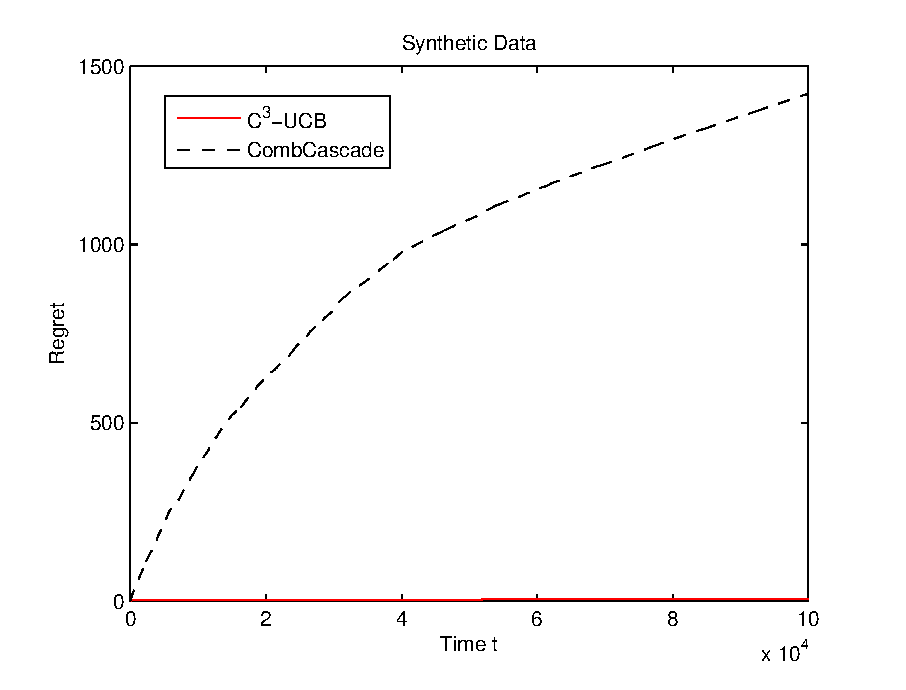
\includegraphics[height = 3 cm, width = 3.95 cm]{synD-T5-L100-K4-1.eps}}
	\subfigure[Disjunctive, $\gamma=0.9$]{
		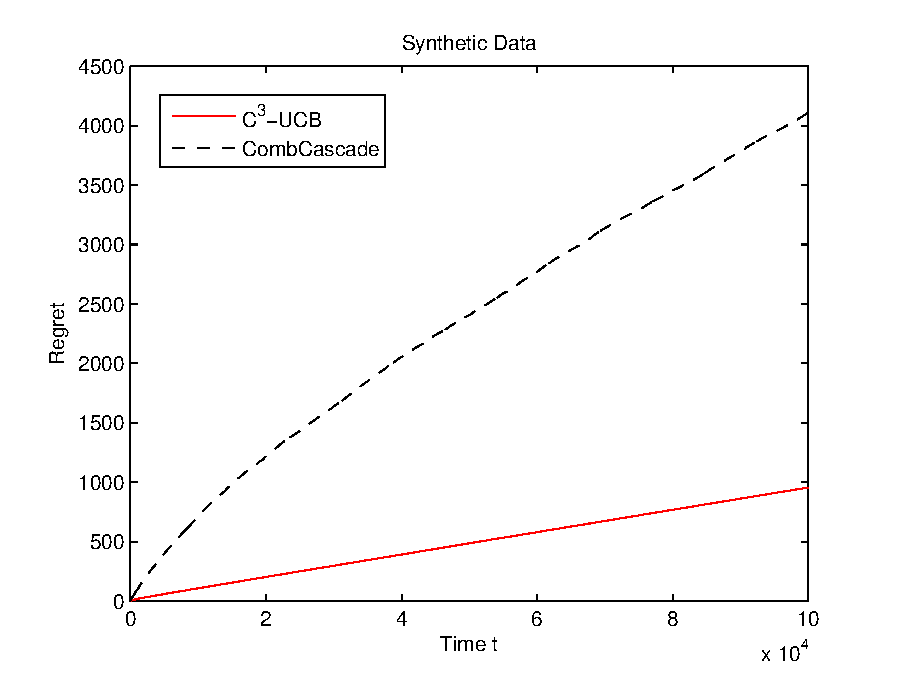
\includegraphics[height = 3 cm, width = 3.95 cm]{synD-T5-L100-K4-9.eps}}\\
	\subfigure[Conjunctive, $\gamma=1$ ]{
		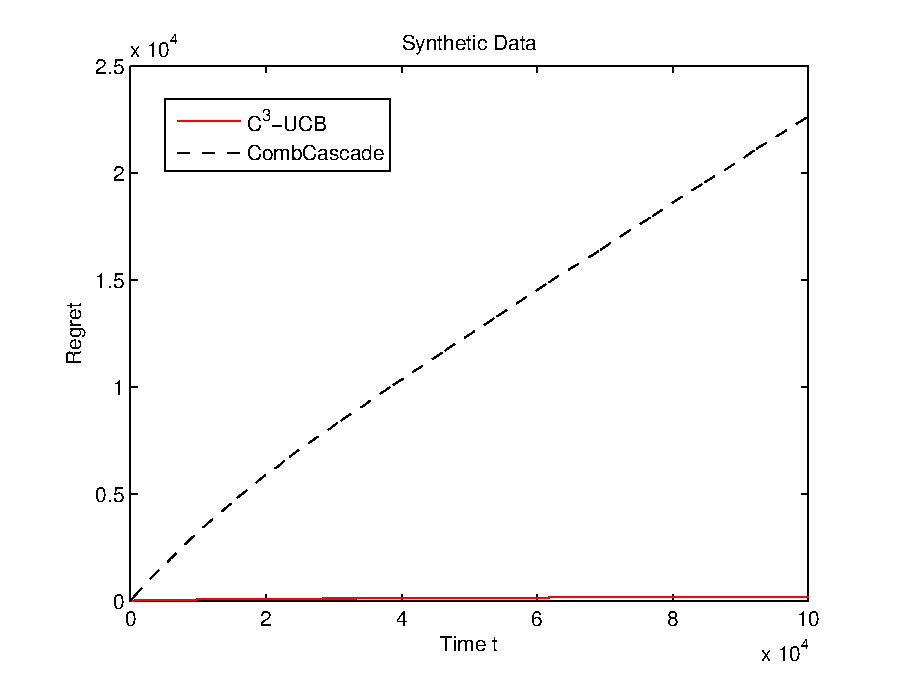
\includegraphics[height = 3 cm, width = 3.95 cm]{synC-T5-L100-K4-1.eps}}
	\subfigure[Conjunctive, $\gamma=0.9$ ]{
		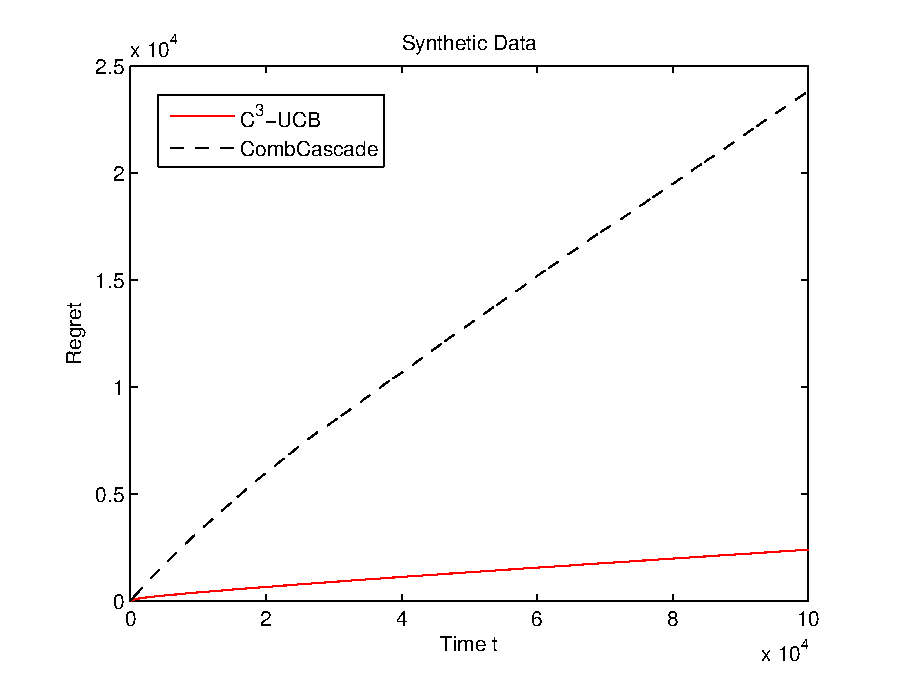
\includegraphics[height = 3 cm, width = 3.95 cm]{synC-T5-L100-K4-9.eps}}
	\caption{Synthetic Data Set, L=100, K=4, d=10}
	\label{fig:synthetic} % 用于交叉引用
\end{figure}



\section{Experiments}

We evaluate our algorithm, $C^3$-UCB, in a synthetic setting and two real applications. The results are compared with {\it CombCascade}, the study most related to ours, and demonstrate the advantage to involve contextual information and position discounts. In experiments, we set the position discounts $\gamma_k$ to be $\gamma^{k-1}$ for some $\gamma$. 

\subsection{Synthetic Data}
\label{sec:ExpSyn}

In the first experiment, we compare $C^3$-UCB to {\it CombCascade} on synthetic problems. This problem is a contextual cascading bandit with $L=100$ items and $K=4$, where at each time $t$ the agent recommends $K$ items to the user. At first, we randomly choose a $\theta \in \RR^{d-1}$ with $\|\theta \|_2 = 1$ and let $\theta_* = (\frac{\theta}{2}, \frac{1}{2})$. Then at each time $t$, we randomly assign $x'_{t,a} \in \RR^{d-1}$ with $\|x'_{t,a}\|_2 = 1$ to arm $a$ and use $x_{t,a} = (x'_{t,a}, 1)$ to be the contextual information for arm $a$. This processing will guarantee the inner product $\theta_*^{\top}x_{t,a} = \frac{1}{2}(\theta^{\top}x'_{t,a} + 1) \in [0,1]$. Next we generate the weight for arm $a$ at time $t$ by a random sample from the Bernoulli distribution with mean $\theta_*^{\top}x_{t,a}$.

We conduct experiments in four settings. Under each setting, the learning agent chooses a set of $K$ items out of $L$ ground items. The first two are of disjunctive objective where the learning agent observes a prefix of the chosen $K$ items until the first one with weight $1$; the last two are of conjunctive objective where the learning agent observes from the first item until the first one with weight $0$. Notice that with $\gamma \leq 1$, the oracle selects a set of $K$ items with highest UCBs in their decreasing order. The regrets are shown in Fig.~\ref{fig:synthetic} and our algorithm outperforms {\it CombCascade} algorithm because they do not make use of the contextual information.


\subsection{Movie Recommendation}
\label{sec:movie}

\begin{figure}
	\centering
	\subfigure[$\gamma = 1$]{
		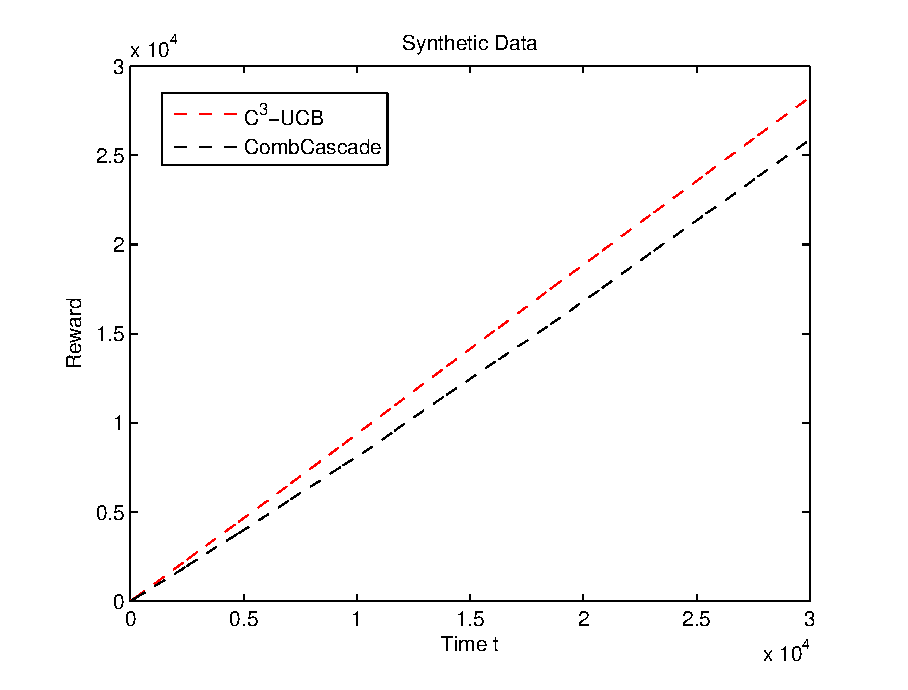
\includegraphics[height = 3cm, width = 3.95 cm]{movieT30000-L200-K4-1.eps}}
	\subfigure[$\gamma = 0.9$]{
		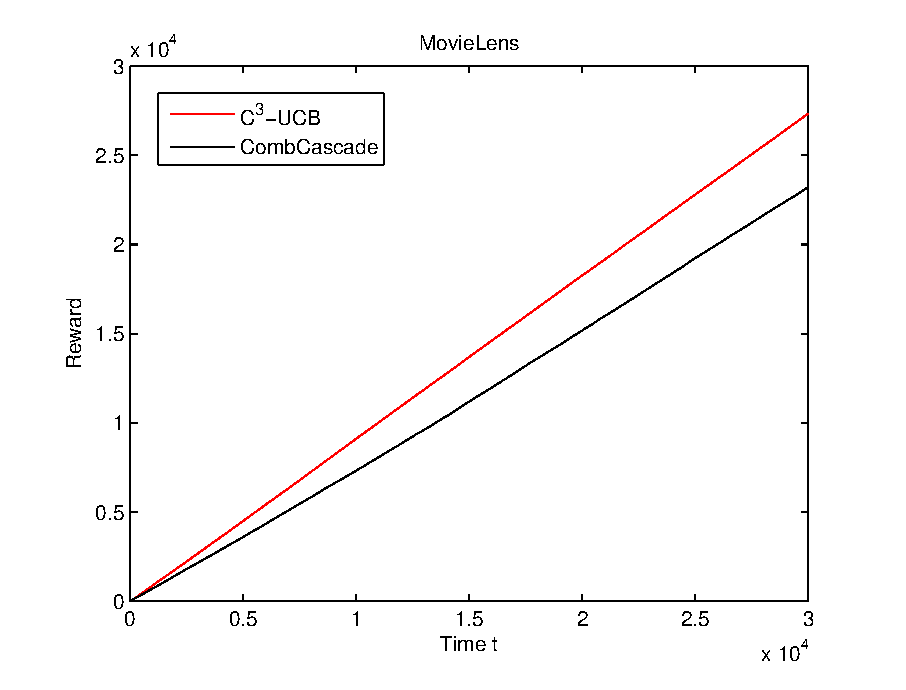
\includegraphics[height = 3cm, width = 3.95 cm]{movieT30000-L200-K4-9.eps}}
	\caption{Rewards on MovieLens, $L=200$, $K=4$, $d=5$}
	\label{fig:movielens} % 用于交叉引用
\end{figure}

In this experiment, we evaluate $C^3$-UCB on movie recommendation with data set {\it MovieLens} \cite{lam2013movie} of 2015.

The learning problem is formulated as follows. There is a big sparse matrix $A \in \{0,1\}^{N_1 \times N_2}$ where $A(i,j) = 1$ denotes user $i$ has watched movie $j$. Next, we split $A$ as $H + F$ by putting $1$-entry in $A$ to $H$ or $F$ according to a Bernoulli distribution $\sim \mathrm{Ber}(p)$ for some fixed $p$. We regard $H$ as known information about history ``what users have watched'' and regard $F$ as future criterion. We use $H$ to derive feature vectors of both users and movies by SVD decomposition, $H = USM^{\top}$ where $U = (u_1; ...;u_{N_1})$ and $M = (m_1;...;m_{N_2})$. At every time $t$, we randomly choose a user $I_t \in [N_1]$. Then in the same spirit of \cite{li2010contextual}, we use $x_{t,j} = u_{I_t}m_j^{\top}$, the outer product of $u_{I_t}$ and $m_{j}$, as the contextual information for each movie $j$. The real weight of movie $j$ at time $t$, $\bw_t(j)$, is $F(I_t,m)$.

For this experiment, we randomly choose $L=200$ movies and recommend $K=4$ movies at each time. We experiment with both $\gamma=1$ (no position discount) and $\gamma=0.9$, and compare our algorithm with {\it CombCascade}. The results for rewards are shown in Fig.\ref{fig:movielens}. The rewards of our algorithms are higher than those of {\it CombCascade} by $9.2\%$ and $17.74\%$ (for $\gamma = 1$ and $0.9$, respectively), which demonstrate the advantage to involve contextual information in real applications.

\subsection{Network Routing Data}

In the last experiment, we evaluate $C^3$-UCB on network routing problem with {\it RocketFuel} dataset \cite{spring2004measuring}.

The ground set $E$ is the set of links in the network. Before learning, the environment randomly chooses a $d$-dimensional vector $\theta_* \in [0,1]^d$. At each time $t$, a pair of source and destination nodes are randomly chosen and the feasible action set $\cS_t$ at time $t$ contains all simple paths between the source and destination. Any edge $a$ in the set $\cS_t$ is assigned with a random $d$-dimensional contextual information vector $x_{t,a}$. Notice here both $\theta$ and $x$ have been processed like in Section \ref{sec:ExpSyn} such that $\theta_*^{\top}x \in [0,1]$. The weight for each edge $a$ is a sample from Bernoulli distribution with mean $\theta_*^{\top}x_{t,a}$. Then the learning agent recommends a feasible path $A = (a_1,...,a_{|A|})$ between source and destination nodes to maximize the expected reward in the conjunctive objective. We experiment on different position discounts. The regrets are shown in Fig.~\ref{fig:network} (a), (b). 

Another experiment is conducted on the network with latency, where the latency on an edge is an exponential random variable with mean $\theta_{\ast}^{\top}x$ and the reward is $1$ if the latency is less than a tolerance $\tau = 0.75$. The comparison of the cumulative rewards of our algorithm with {\it CombCascade} is shown in Fig.~\ref{fig:network} (c).

We also conduct an experiment on the influence of $\gamma$ to the regret. In recommendations, the position discounts represent users' satisfaction and the learning agent may not know its true value. Suppose the true position discount $\gamma^{\ast} = 0.9$ and the learning agent sets $\gamma$ by her experience. We experiment on different $\gamma \in \{0.8, 0.82, \ldots, 0.98, 1.0\}$ with the true criterion $\gamma^{\ast} = 0.9$. The regrets with different $\gamma$'s are illustrated in Fig.~\ref{fig:network}(d), from which it can be seen that the regret is minimized around the true $\gamma^{\ast}$. The big gap between the regret at $\gamma = 1$ and $\gamma^{\ast} = 0.9$ shows that it significantly benefits by exploiting position discounts in the model when such discounts indeed exist in applications.

\begin{figure}
	\centering
	\subfigure[Network 1239, $\gamma=1$]{
		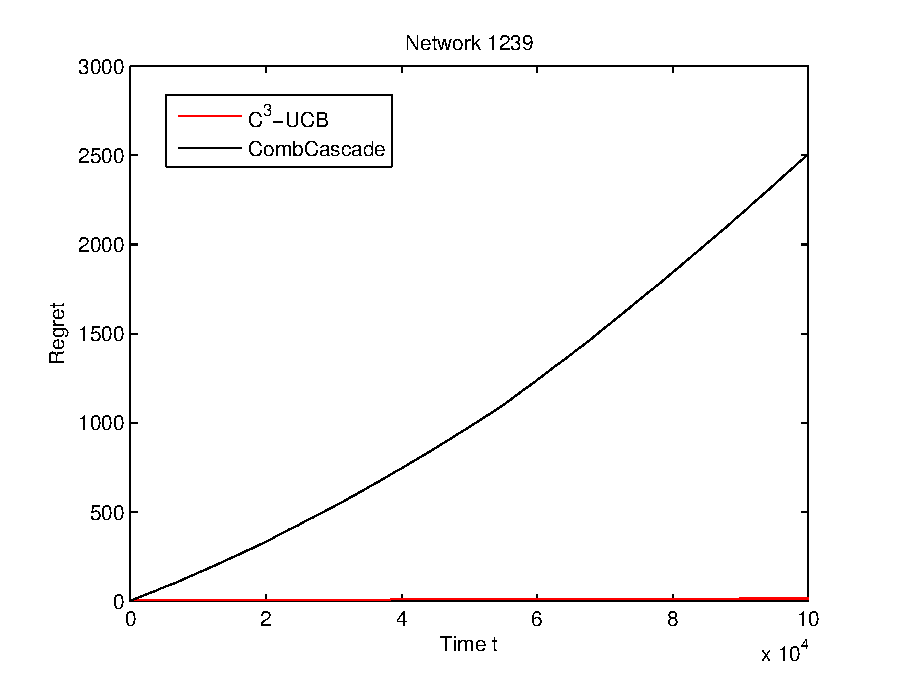
\includegraphics[height = 3 cm, width = 3.95 cm]{isp1239-T5-k100-1.eps}}
	\subfigure[Network 3356, $\gamma = 0.9$]{
		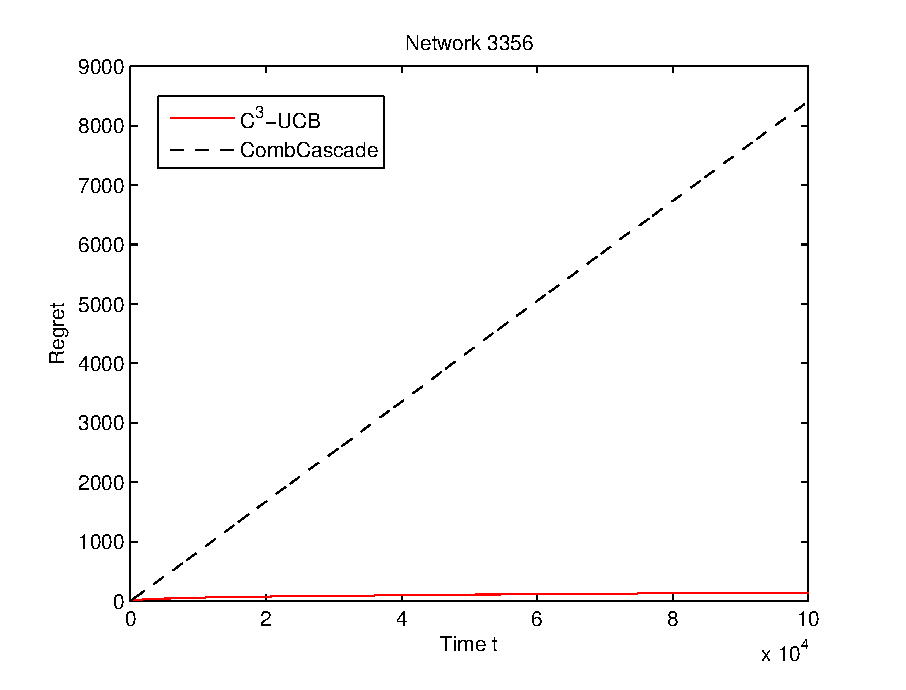
\includegraphics[height = 3 cm, width = 3.95 cm]{isp3356-T5-k100-9.eps}}\\
	\subfigure[Rewards on network 1755 with latency, $\gamma = 0.9$ ]{
		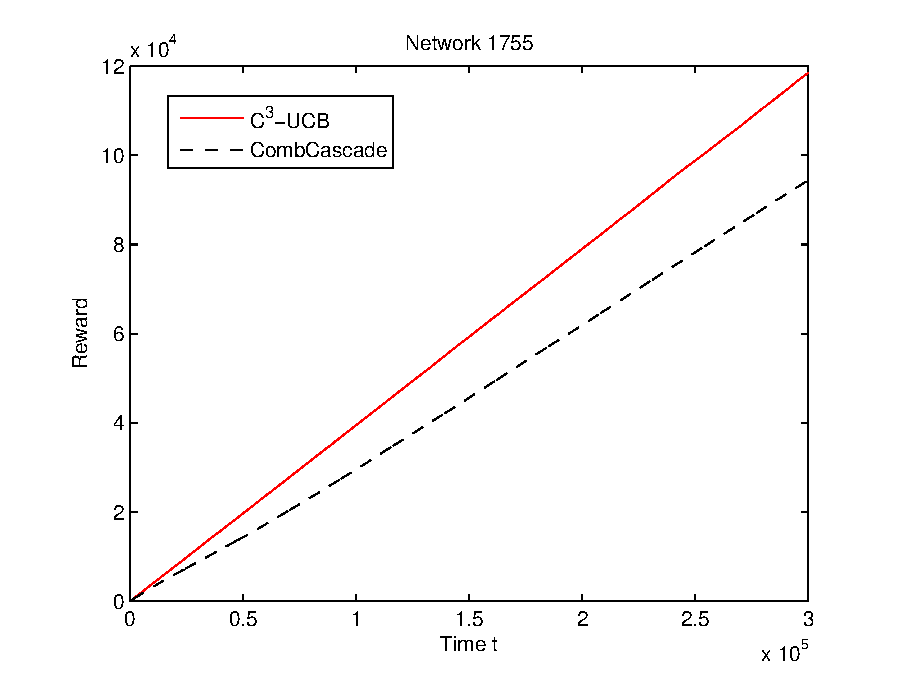
\includegraphics[height = 3 cm, width = 3.95 cm]{isp1755-T300000-gamma9-latency.eps}}
	\subfigure[Comparison of different $\gamma$ with true $\gamma^{\ast} = 0.9$, $n = 10000$ ]{
		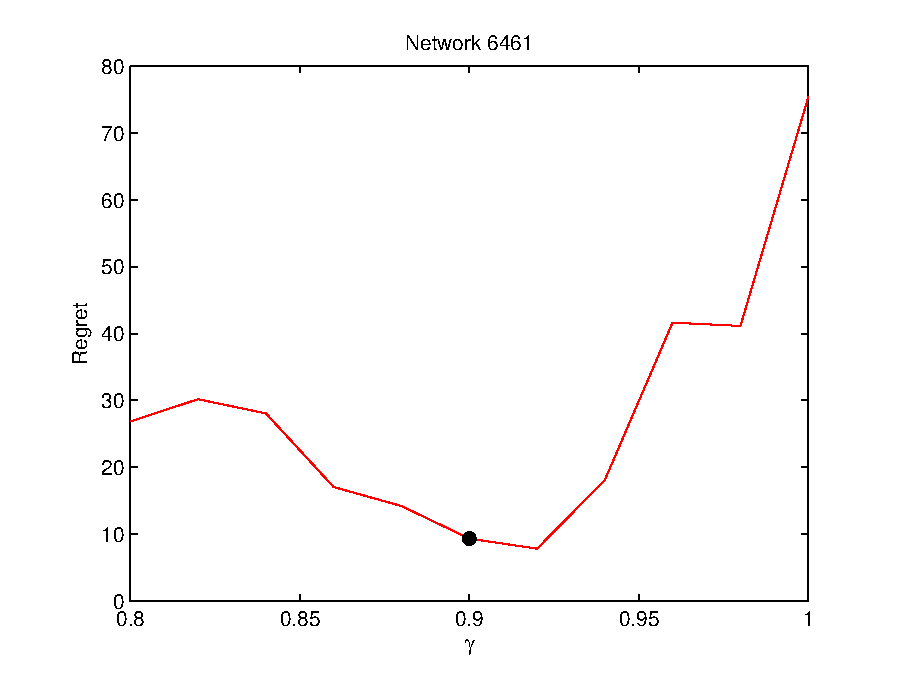
\includegraphics[height = 3 cm, width = 3.95 cm]{network-gamma-with-point.eps}}
	\caption{Network, $d=10$}
	\label{fig:network} % 用于交叉引用
\end{figure}


% we randomly generate a pair of starting and ending nodes, and the learning agent chooses a routing path between the two nodes to maximize the expected reward with position discount.

%  and the corresponding latency follows exponential distribution with mean $1-\theta^{\top}x$, which has been scaled into $[0,1]$. We call the latency is {\it high} if it is larger than a threshold $\tau$. 
% $$
% \prod_{k=1}^{|A|} (1- \exp(-\frac{\tau}{1-\theta^{\top}x_{t,a_k}})).
% $$
% Notice that the expression is not of the form $\prod_{k=1}^{|A|}\theta_*^{\top}x_{t,a_k}$ in our model. However, our algorithm could also apply to it.


\section{Conclusions}

In this paper, we propose contextual combinatorial cascading bandits with position discounts, where each action is an ordered list and only a prefix of the action is observed each time. We propose a C$^3$-UCB algorithm and prove a cumulative regret bound for general reward functions and two special reward functions. The experiments conducted demonstrate the advantage to involve contextual information and position discounts. In future, we would like to investigate on lower bounds of the regret and cascading on general graphs.


% In the unusual situation where you want a paper to appear in the
% references without citing it in the main text, use \nocite
%\nocite{langley00}

\newpage
\bibliography{cascade_reference}
\bibliographystyle{icml2016}

\newpage

\appendix

\section{Proof of Theorem~\ref{thm:main}}

The following lemma provides the important result on the regret at each time $t$ in terms of feature vectors of base arms at the time.

\begin{lemma} %lem:DeltaEstimate
	\label{lem:DeltaEstimate}
	For any time $t$ and $\bA_t = (\ba_1^t, \ldots, \ba_{\abs{A}}^t)$, if $f$ satisfies the two assumptions of monotonicity and $B$-Lipschitz continuity, 
	%and $f(A_t^*, \bU_t) \leq f(A, \bU_t)$, 
	then we have
	$$
		R^{\alpha}(t, \bA_t) \leq 2B \sum_{k=1}^{\abs{\bA_t}} \gamma_k \bbeta_{t-1}(\delta)\norm{x_{t, \ba_k}}_{\bV_{t-1}^{-1}}.
	$$
\end{lemma}
\begin{proof}
	By Lemma \ref{lem:estimateU}, $w_t \leq \bU_t$. Then
	\begin{align*}
		f(\bA_t, \bU_t) \geq \alpha f(\bA^{\bU_t}, \bU_t) \geq \alpha f(A_t^*, \bU_t) \geq \alpha f(A_t^*, w_t),
	\end{align*}
	where $\bA^{\bU_t} = \argmax_{A \in \cS} f(A, \bU_t)$. The first inequality is because we choose $\bA_t$ by the $\alpha$-approximation oracle with input $\bU_t$; the second inequality is because the maximum of $f(\bA^{\bU_t}, \bU_t)$ given $\bU_t$; the third inequality is by the monotonicity of $f$ and the property $\bU_t \geq w_t$. Then
	\begin{align*}
		R^{\alpha}(t, \bA_t) = &\alpha f(A_t^*, w_t) - f(\bA_t, w_t) \\
		\leq &f(\bA_t, \bU_t) - f(\bA_t, w_t).
	\end{align*}
	By Lipschitz continuity of $f$ and Lemma \ref{lem:estimateU},
	\begin{align*}
		f(\bA_t, \bU_t) &\leq f(\bA_t, w_t) + B \sum_{k=1}^{\abs{\bA_t}} \gamma_k \abs{\bU_t(\ba_k^t) - w_t(\ba_k^t)}\\
		& \leq f(\bA_t, w_t) + 2B \sum_{k=1}^{\abs{\bA_t}} \gamma_k\bbeta_{t-1}(\delta)\norm{x_{t, \ba_k^t}}_{\bV_{t-1}^{-1}}.
	\end{align*}
	Then we have
	\begin{align*}
		R^{\alpha}(t, A) \leq &f(\bA_t, \bU_t) - f(\bA_t, w_t) \\
		\leq &2B \sum_{k=1}^{\abs{\bA_t}} \gamma_k \bbeta_{t-1}(\delta)\norm{x_{t, \ba_k^t}}_{\bV_{t-1}^{-1}}.
	\end{align*}
\end{proof}

Notice that the upper bound of $R^{\alpha}(t, \bA_t)$ is in terms of all base arms of $\bA_t$. However, it is hard to estimate an upper bound for $\sum_{t=1}^T \sum_{k=1}^{\abs{\bA_t}} \norm{ x_{t, \ba_k^t} }_{ \bV_{t-1}^{-1} }$ because $\bV_t$ only contains information of observed base arms. Thus we need the following lemma.

\begin{lemma} %lem:DeltaEsimateWithP*
	\label{lem:DeltaEsimateWithP*}
	Suppose the Ineq.\eqref{eq:estimateTheta} holds for time $t-1$. Then
	$$
	\EE[R^{\alpha}(t, \bA_t) | \cH_t] \leq \frac{2B}{p^*} \EE \left[ \left.\bbeta_{t-1}(\delta) \sum_{k=1}^{\bO_t}\norm{\gamma_k x_{t,\ba_k^t}}_{\bV_{t-1}^{-1}} \right| \cH_t \right].
	$$
\end{lemma}
\begin{proof}
	\begin{align}
		&\EE[R^{\alpha}(t, \bA_t)|\cH_t]  \nonumber \\
		=& \EE \left[ \left. R^{\alpha}(t, \bA_t) \EE \left[ \left. \frac{1}{p_{t, \bA_t}} \bOne\{\bO_t = \abs{\bA_t}\} \right| \bA_t \right]  \right| \cH_t \right] \label{eq:addOt}\\
		=& \EE \left[ \left. R^{\alpha}(t, \bA_t) \frac{1}{p_{t, \bA_t}} \bOne\{\bO_t = \abs{\bA_t}\}  \right| \cH_t \right] \label{eq:removeE}\\
		\leq &\frac{1}{p^{\ast}} \EE \left[ \left. R^{\alpha}(t, \bA_t) \bOne\{\bO_t = \abs{\bA_t}\}  \right| \cH_t \right] \label{eq:relaxpstar}\\
		\leq &\frac{2B}{p^{\ast}} \EE \left[ \left. \sum_{k=1}^{\abs{\bA_t}} \gamma_k \bbeta_{t-1}(\delta)\norm{x_{t,a_k}}_{\bV_{t-1}^{-1}} \bOne\{\bO_t = \abs{\bA_t}\}  \right| \cH_t \right] \label{eq:useradiusbound}\\
		\leq &\frac{2B}{p^{\ast}} \EE \left[ \left. \sum_{k=1}^{\bO_t} \gamma_k \bbeta_{t-1}(\delta)\norm{x_{t,a_k}}_{\bV_{t-1}^{-1}} \right| \cH_t \right]. \label{eq:relaxindicator}
	\end{align}
	Eq.\eqref{eq:addOt} is because when $\bA_t$ is fixed, $p_{t, \bA_t}$ is the probability of $\bO_t = \abs{\bA_t}$, and thus the inner expectation is $1$. Eq.\eqref{eq:removeE} is because when the history $\cH_t$ is fixed, $\bA_t$ is fixed by the deterministic algorithm C$^3$-UCB, and thus there is no need to write the conditional expectation. Ineq.\eqref{eq:relaxpstar} is because $p_{t,\bA_t} \geq p^*$ by definition. Ineq.\eqref{eq:useradiusbound} is by Lemma \ref{lem:DeltaEstimate} and the fact $f(A_t^*, \bU_t) \leq f(\bA_t, \bU_t)$, which is true because algorithm C$^3$-UCB selects action $\bA_t$ as the best action with respect to $\bU_t$. Ineq.\eqref{eq:relaxindicator} is by simply arguing on the two cases for the indicator function $\bOne\{\bO_t = \abs{\bA_t}\}$.
\end{proof}

From the above lemma, we can bound the regret at time $t$ in terms of the observed base arms, for which we further bound in Lemma~\ref{lem:SumXiEstimateInDet}.
But before that, we need the following technical lemma.

\begin{lemma} %lem:detTech
  \label{lem:detTech}
  Let $x_i \in \RR^{d \times 1}, 1 \leq i \leq n$. Then we have
  $$
    \det\left(I + \sum_{i=1}^n x_i x_i^{\top}\right) \geq 1 + \sum_{i=1}^n \norm{x_i}_2^2.
  $$
\end{lemma}
\begin{proof}
  Denote the eigenvalues of $I + \sum_{i=1}^n x_i x_i^{\top}$ by $1+\alpha_1,...,1+\alpha_d$ with $\alpha_j \geq 0$, $1\leq j\leq d$. Then
  \begin{align*}
    &\det(I + \sum_{i=1}^n x_i x_i^{\top})= \prod_{j=1}^d (1 + \alpha_j)\\
    \geq& 1 +\sum_{j=1}^d \alpha_j =1-d + \sum_{i=1}^d (1+\alpha_i) \\
    =&1-d + \trace(I + \sum_{i=1}^n x_i x_i^{\top})= 1-d + d + \sum_{i=1}^n \norm{x_i}_2^2\\
    =&1 + \sum_{i=1}^n \norm{x_i}_2^2.
  \end{align*}
\end{proof}


\begin{lemma} % lem:SumXiEstimateInDet
  \label{lem:SumXiEstimateInDet}
  \CLemmaSumXiEstimateInDet
\end{lemma}
\begin{proof}
	\begin{align}
	&\det(\bV_t) = \det\left(\bV_{t-1} + \sum_{k=1}^{\bO_t} (\gamma_k x_{t,\ba_k^{t}})(\gamma_k x_{t, \ba_k^{t}}^{\top}) \right) \nonumber \\
	=&\det(\bV_{t-1}) \notag \\
	&~~~\cdot \det \left(I + \sum_{k=1}^{\bO_t} \gamma_k \bV_{t-1}^{-1/2}x_{t,\ba_{k}^{t}} (\gamma_k \bV_{t-1}^{-1/2}x_{t,\ba_{k}^{t}})^{\top} \right) \label{eq:Vfactor}\\
	\geq& \det(\bV_{t-1}) \left(1 + \sum_{k=1}^{\bO_t} \norm{\gamma_k x_{t,\ba_k^t}}_{\bV_{t-1}^{-1}}^2 \right) \label{eq:detGeq} \\
	\geq& \det(\lambda I)\prod_{s=1}^{t} \left(1 + \sum_{k=1}^{\bO_s} \norm{\gamma_k x_{s,\ba_k^s}}_{\bV_{s-1}^{-1}}^2 \right), \label{eq:repeatV}
	\end{align}
	where Eq.\eqref{eq:Vfactor} is by the fact that $V+U = V^{1/2} (I + V^{-1/2} U V^{-1/2}) V^{1/2}$ for a symmetric positive definite matrix $V$, Ineq.\eqref{eq:detGeq} is due to Lemma \ref{lem:detTech}, and Ineq.\eqref{eq:repeatV} is by repeatedly applying Ineq.\eqref{eq:detGeq}.
	
	Because
	$$
	\norm{\gamma_k x_{s,\ba_k^s}}_{\bV_{s-1}^{-1}}^2 \leq \norm{\gamma_k x_{s,\ba_k^s}}_2^2/\lambda_{\min}(\bV_{s-1}) \leq \gamma_k^2 /\lambda,
	$$
	where $\lambda_{\min}(\bV_{s-1})$ is the minimum eigenvalue of $\bV_{s-1}$,  we have 
	$$
	\sum_{k=1}^{\bO_s} \norm{\gamma_k x_{s,\ba_k^s}}_{\bV_{s-1}^{-1}}^2 \leq \frac{1}{\lambda} \sum_{k=1}^{K} \gamma_k^2 = C_\gamma /\lambda \leq 1
	$$
	Using the fact that $ 2\ln(1+u) \geq u$ for any $u \in [0,1]$, we get
	\begin{align*}
	&\sum_{s=1}^t \sum_{k=1}^{\bO_s}\norm{\gamma_k x_{s,\ba_{k}^s}}_{\bV_{s-1}^{-1}}^2 \\
	\leq &2\sum_{s=1}^t\ln \left(1 + \sum_{k=1}^{\bO_s} \norm{\gamma_k x_{s,\ba_k^s}}_{\bV_{s-1}^{-1}}^2 \right)\\
	= &2 \ln \prod_{s=1}^{t} \left(1 + \sum_{k=1}^{\bO_s} \norm{\gamma_k x_{s,\ba_k^s}}_{\bV_{s-1}^{-1}}^2 \right) \\
	\le& 2 \ln \left(\frac{\det(\bV_t)}{\det(\lambda I)} \right),
	\end{align*}
	where the last inequality is from Ineq.\eqref{eq:repeatV}.
\end{proof}

Finally the last lemma bounds $\det(\bV_t)$.

\begin{lemma} % det(V_t)
	\label{lem:detVt}
	\CLemmaDetVt
\end{lemma}
\begin{proof}
	To prove $\det(\bV_t)$ is increasing with respect to $t$, it is enough to prove that
	$$
	\det(V + xx^{\top}) \geq \det(V),
	$$
	for any symmetric positive definite matrix $V \in \RR^{d \times d}$ and column vector $x \in \RR^{d\times 1}$. In fact,
	\begin{align*}
	&\det(V + xx^{\top}) \\
	=& \det(V) \det(I + V^{-1/2}x x^{\top} V^{-1/2})\\
	=& \det(V) \det(1 + \norm{V^{-1/2}x}^2)\\
	\geq &\det(V).
	\end{align*}
	The second equality above is due to Sylvester's determinant theorem, which states that $\det(I + AB) = \det(I +BA)$.
	
	Let the eigenvalues of $\bV_t$ be $\lambda_1, \ldots, \lambda_d > 0$. Then
	\begin{align*}
	\det(\bV_t) &= \lambda_1 \cdot \cdots \cdot \lambda_d \\
	&\leq  \left( \frac{\lambda_1 + \ldots + \lambda_d}{d} \right)^d = (\trace(\bV_t)/d)^d.
	\end{align*}
	Also,
	\begin{align*}
	&\trace(\bV_t)\\
	=& \trace(\lambda I) + \sum_{s=1}^t \sum_{k=1}^{\bO_s} \gamma_k^2 \trace(x_{s,\ba_k^s} x_{s,\ba_k^s}^{\top})\\	
	=& d \lambda + \sum_{s=1}^t \sum_{k=1}^{\bO_s} \gamma_k^2 \norm{x_{s,\ba_k^s}}_2^2\\
	\leq& d \lambda + \sum_{s=1}^t\sum_{k=1}^{K}\gamma_k^2 = d \lambda + t C_\gamma.
	\end{align*}
	Thus we have $\det(\bV_t) \leq (\lambda + C_\gamma t/d)^d.$
\end{proof}

Lemma \ref{lem:SumXiEstimateInDet} and Lemma \ref{lem:detVt} combined imply Lemma \ref{lem:XNormSumEst}. Now we are ready to prove the main theorem.

\begin{proof}[ of Theorem \ref{thm:main}]
	Suppose Ineq.\eqref{eq:estimateTheta} holds for all time $t$, which is true with probability $1-\delta$. Then with probability $1-\delta$, we have
	\begin{align}
	&R^{\alpha}(n) = \EE \left[\sum_{t=1}^{n} \EE[R^{\alpha}(t, \bA_t) | \cH_t] \right] \notag\\
	&\leq \EE\left[\sum_{t=1}^{n} \frac{2B}{p^*} \EE \left[ \left. \bbeta_{t-1}(\delta) \sum_{k=1}^{\bO_t}\norm{\gamma_k x_{t,\ba_k^t}}_{\bV_{t-1}^{-1}}\right| \cH_t \right] \right] \label{eq:pfMdeltaEst}\\
	&\leq \EE\left[\sum_{t=1}^{n} \frac{2B}{p^*} \bbeta_{n}(\delta) \EE \left[ \left. \sum_{k=1}^{\bO_t}\norm{\gamma_k x_{t,\ba_k^t}}_{\bV_{t-1}^{-1}} \right| \cH_t \right] \right] \label{eq:pfMbeta}\\
	&\leq \EE \left[\frac{2B}{p^*} \bbeta_n(\delta) \sqrt{\left(\sum_{t=1}^{n} \bO_t\right) \left( \sum_{t=1}^{n} \sum_{k=1}^{\bO_t}\norm{\gamma_k x_{t,\ba_k^t}}_{\bV_{t-1}^{-1}}^2 \right)} \right ]  \label{eq:pfMmeanEq}\\
	&\leq \EE\left[\frac{2B}{p^*} \left( R \sqrt{ \ln \left( \frac{\det(\bV_n)}{\lambda^d / n} \right)} + \sqrt{\lambda} \right) \right. \notag\\
	& \left. \qquad \qquad \cdot \sqrt{nK \cdot 2\ln \left(\frac{\det(\bV_n)}{\lambda^d} \right)} \right] \label{eq:pfMsumXi}\\
	&\leq \frac{2\sqrt{2}B}{p^*} \left(R\sqrt{ \ln[ (1 + C_\gamma n/(\lambda d))^d n ]} + \sqrt{\lambda} \right) \notag\\
	&\qquad \qquad \cdot \sqrt{nKd\ln(1 + C_\gamma n/(\lambda d))}. \label{eq:pfMdetEst}
	\end{align}
	Ineq.\eqref{eq:pfMdeltaEst} is by Lemma \ref{lem:DeltaEsimateWithP*}. 
	Ineq.\eqref{eq:pfMbeta} is because $\bbeta_{t}(\delta)$ is increasing with respect to $t$, derived by the definition of $\bbeta_t(\delta)$ (Eq.\eqref{eq:definebeta}) and Lemma \ref{lem:detVt}. 
	Ineq.\eqref{eq:pfMmeanEq} is by the mean inequality. 
	Ineq.\eqref{eq:pfMsumXi} is because of the definition of $\bbeta_t(\delta)$ (Eq.\eqref{eq:definebeta}) and Lemma \ref{lem:SumXiEstimateInDet}. 
	And the last Ineq.\eqref{eq:pfMdetEst} is because estimate of $\det(\bV_t)$ by Lemma \ref{lem:detVt}.
	
	Also $R^{\alpha}(n) \leq \alpha n$ and $\delta = \frac{1}{\sqrt{n}}$. We have 
	\begin{align*}
		R^{\alpha}(n) &\leq \frac{2\sqrt{2}B}{p^*} \left(R\sqrt{ \ln[ (1 + C_\gamma n/(\lambda d))^d n ]} + \sqrt{\lambda} \right) \\
		&\qquad \cdot \sqrt{nKd\ln(1 + C_\gamma n/(\lambda d))} + \alpha \sqrt{n}.
	\end{align*}
\end{proof}

\section{Proof of Corollary~\ref{cor:or}}

In this section, we prove the expected reward function
$$
f(A,w) = \sum_{k = 1}^{\abs{A}} \gamma_{k} \prod_{i=1}^{k-1} (1 - w(a_i)) w(a_k),
$$
where $A = (a_1, \ldots, a_{|A|})$, defined in~Eq.\eqref{eq:OrRewardFunc}, satisfies the properties of monotonicity and $1$-Lipschitz continuity.

\begin{lemma}[monotonicity]
	\label{lem:orMonotonicity}
	Suppose $1 \geq \gamma_1 \geq \cdots \geq \gamma_K \geq 0$. Then $f(A, w)$ is increasing with respect to $w$, that is, if $w \leq w' \in [0,1]^E$, then for any $A \in \prod^{\leq K}$, it holds that
	$$
	f(A, w) \leq f(A, w').
	$$
\end{lemma}
\begin{proof}
	Without the loss of generality, we prove for the case of $A = (1, \ldots, m)$, where $1 \leq m \leq K$. Denote $w = (w_a)_{a \in E}$ and $w' = (w'_a)_{a \in E}$. First, for $1 \leq k \leq m$, we have
	\begin{align*}
		&\gamma_{k} - \sum_{i=k+1}^m \gamma_i \prod_{j = k + 1}^{i - 1} (1 - w_j') w_i'\\
		\geq &~\gamma_k [1 - \sum_{i=k+1}^m \prod_{j=k+1}^{i-1}(1 - w_j') w_i']\\
		\geq &~\gamma_{k} \cdot 0 = 0.
	\end{align*}
	Then it implies that
	\begin{align*}
		&\gamma_k w_k + (1 - w_k)\sum_{i=k+1}^m \gamma_i \prod_{j=k+1}^{i-1}(1 - w_j') w_i'\\
		\leq &\gamma_k w_k' + (1 - w_k')\sum_{i=k+1}^m \gamma_i \prod_{j=k+1}^{i-1}(1 - w_j') w_i'.\\
	\end{align*}
	Therefore, 
	\begin{align*}
		& f(A; w_1, \dots, w_k, w_{k+1}', \dots, w_m')\\
		=&\sum_{i=1}^{k-1} \gamma_i \prod_{j=1}^{i-1}(1 - w_j) w_i + \prod_{j=1}^{k-1}(1 - w_j) \\
		&\qquad \cdot [\gamma_k w_k + (1 - w_k)\sum_{i=k+1}^m \gamma_i \prod_{j=k+1}^{i-1}(1 - w_j') w_i']\\
		\leq& \sum_{i=1}^{k-1} \gamma_i \prod_{j=1}^{i-1}(1 - w_j) w_i + \prod_{j=1}^{k-1}(1 - w_j) \\
		&\qquad \cdot [\gamma_k w_k' + (1 - w_k')\sum_{i=k+1}^m \gamma_i \prod_{j=k+1}^{i-1}(1 - w_j') w_i']\\
		=&f(A; w_1, \ldots, w_{k-1}, w_{k}', \ldots, w_m').
	\end{align*}
\end{proof}

\begin{lemma}[Lipschitz continuity]
	\label{lem:orLip}
	Suppose $0 \leq \gamma_k \leq 1, k \leq K$. Let $w, w'\in [0,1]^{E}$. Then
	$$
	|f(A, w) - f(A, w')| \leq \sum_{k=1}^{|A|} \gamma_k |w(a_k) - w'(a_k)|,
	$$
	where $A = (a_1, \ldots, a_{|A|})$.
\end{lemma}
\begin{proof}
	Without the loss of generality, we prove for the case of $A = (1, \ldots, m)$, where $1 \leq m \leq K$. Denote $w = (w_a)_{a \in E}$ and $w' = (w'_a)_{a \in E}$. First, suppose $w \leq w'$ and $w' = w + v$.
	
	We prove this by induction. It holds obviously for $m = 1$. Suppose it holds for $m$. Then
	\begin{align*}
		&f(A^{(m+1)}, w')\\
		=&f(A^{(m)}, w') + \gamma_{m+1}\prod_{k=1}^m(1 - w'_k) w'_{m+1}\\
		\leq &f(A^{(m)}, w') +  \gamma_{m+1} \prod_{k=1}^m(1 - w_k) (w_{m+1} + v_{m+1})\\
		\leq &f(A^{(m)}, w) + \sum_{k=1}^m \gamma_k v_k \\
		&\qquad + \gamma_{m+1} \prod_{k=1}^m(1 - w_k) w_{m+1} + \gamma_{m+1} v_{m+1}\\
		=& f(A^{(m+1)}, w) + \sum_{k=1}^{m+1} \gamma_k v_k.
	\end{align*}
	So it holds for $m+1$.
	
	For general $w,w' \in [0,1]^L$, by Lemma \ref{lem:orMonotonicity}, we have
	$$
	f(A, w\wedge w') \leq \{f(A, w), f(A, w') \}\leq f(A, w\vee w'),
	$$
	where 
	$$
	(w\wedge w')_k = \min\{w_k, w'_k\}, ~ (w\vee w')_k = \max\{w_k, w'_k\}.
	$$
	Then
	\begin{align*}
		&|f(A,w) - f(A,w')| \leq f(A, w\vee w') - f(A, w\wedge w')\\
		\leq & \sum_{k=1}^{|A|} \gamma_k [(w\vee w')(a_k) - (w\wedge w')(a_k)]\\
		=& \sum_{k=1}^{|A|} \gamma_k |w(a_k) - w'(a_k)|
	\end{align*}
\end{proof}

We have proved the monotonicity and Lipschitz continuity of expected reward function $f$. Then the corollary follows Theorem \ref{thm:main}.

\section{Proof of Theorem~\ref{thm:and}}

In this section, we prove Theorem \ref{thm:and}. Recall the expected reward function is
$$
f(A,w) = \sum_{k = 1}^{\abs{A}} (1 - \gamma_k) \prod_{i = 1}^{k - 1} w(a_i)(1 - w(a_k)) + \prod_{i=1}^{\abs{A}}w(a_i),
$$
where $A = (a_1, \ldots, a_{|A|})$, as defined in~Eq.\eqref{eq:AndRewardFunc}. First, similar to last section, we prove this reward function satisfies the properties of monotonicity and $1$-Lipschitz continuity.

\begin{lemma}[monotonicity]
	\label{lem:andMonotonicity}
	Suppose $1 \geq \gamma_1 \geq \cdots \geq \gamma_K \geq 0$. Then $f(A, w)$ is increasing with respect to $w$; that is, if $w \leq w' \in [0,1]^E$, then for any $A \in \prod^{\leq K}$, it holds that
	$$
	f(A, w) \leq f(A, w').
	$$
\end{lemma}
\begin{proof}
	Denote $A = (a_1, \ldots, a_{|A|})$. Because
	\begin{align*}
	&1 - f(A, 1-w) \\
	=& 1- \sum_{k = 1}^{\abs{A}} (1 - \gamma_k) \prod_{i = 1}^{k - 1} (1-w(a_i))w(a_k) - \prod_{i=1}^{\abs{A}}(1-w(a_i))\\
	=& \sum_{k = 1}^{\abs{A}} \gamma_{k} \prod_{i=1}^{k-1} (1 - w(a_i)) w(a_k),
	\end{align*}
	then by the proof of Lemma \ref{lem:orMonotonicity} and $1-f(A,1-w)$ is increasing in $w$, we can get $f$ is increasing in $w$.
\end{proof}

\begin{lemma}[Lipschitz continuity]
	\label{lem:andLip}
	Suppose $0 \leq \gamma_k \leq 1, k \leq K$. Let $w, w'\in [0,1]^{L}$. Then
	$$
	|f(A, w) - f(A, w')| \leq \sum_{k=1}^{|A|} \gamma_k |w(a_k) - w'(a_k)|,
	$$
	where $A = (a_1, \ldots, a_{|A|})$.
\end{lemma}
\begin{proof}
	Denote $w = (w_a)_{a \in E}$ and $w' = (w'_a)_{a \in E}$. Similar to the proof of Lemma \ref{lem:orLip}. It is enough to prove when $w \leq w', w' = w + v $ and $A = (1, \ldots, m), m \leq K$. 
	
	We prove this by induction. It holds obviously for $m = 1$. Suppose it holds for $m$. Then
	\begin{align*}
		&f(A^{(m+1)}, w') \\
		= &f(A^{(m)}, w') -\prod_{k=1}^{m} w'_k \\
		&\qquad+ (1-\gamma_{m+1}) (\prod_{k=1}^{m} w'_k) (1 - w'_{m+1})+ \prod_{k=1}^{m+1} w'_k\\
		=& f(A^{(m)}, w') - \gamma_{m+1} (\prod_{k=1}^{m} w'_k) (1 - w'_{m+1})\\
		\leq& f(A^{(m)}, w') - \gamma_{m+1} (\prod_{k=1}^{m} w_k) (1 - w'_{m+1})\\
		\leq& f(A^{(m)}, w') -\gamma_{m+1} (\prod_{k=1}^{m} w_k)  (1 - w_{m+1} - v_{m+1})\\
		\leq& (f(A^{(m)}, w) +  \sum_{k=1}^{m} \gamma_k v_k) \\
		&\qquad - \gamma_{m+1}  (\prod_{k=1}^{m} w_k)(1 - w_{m+1}) + \gamma_{m+1} v_{m+1}\\
		\leq& (A^{(m+1)}, w) + \sum_{k=1}^{m+1} \gamma_k v_k.
	\end{align*}
\end{proof}

The next lemma provides some properties about a prefix of action $A$ in the conjunctive case, which leads to the finding of a prefix $B$ of $A$ with similar regret and probability of full observation as those of $A$, as given in Lemma~\ref{lem:prefixexists}.

\begin{lemma} %lem:prefixRelation
	\label{lem:prefixRelation}
	Suppose $1 = \gamma_1 \geq \gamma_2 \geq \cdots \geq \gamma_K \geq 0$. Let $A = (a_1, ..., a_{\abs{A}})$. Let $B_k = (a_1, ..., a_k), k \leq \abs{A}$ be a prefix of $A$. The expected weights are denoted by $w$. The probability of full observation of $A$, $p_{A}$, can be formulated as
	$$
	p_{A} = \prod_{k=1}^{\abs{A}-1} w_{a_k}.
	$$
	Then for the problem with conjunctive objective and $k < \abs{A}$, we have the following properties:
	\begin{itemize}
		\item[(1)] $f(A, w) \leq (1-\gamma_{\abs{A}}) + \gamma_{\abs{A}} p_{A}$;
		\item[(2)] $f(B_{k+1}, w) \leq f(B_k, w)$;
		\item[(3)] $p_{B_{k+1}} \leq p_{B_k}$;
		\item[(4)] $f(B_k, w) \leq (1-\gamma_{k+1}) + \gamma_{k+1} p_{B_{k+1}}$.
	\end{itemize}
\end{lemma}
\begin{proof}
	Let $m = |A|$. By the definition of $f(A,w)$ in Eq.~\eqref{eq:AndRewardFunc}, we have
	\begin{itemize}
		\item[(1)]
		\begin{align*}
		&f(A,w) \\
		=& \sum_{k = 1}^{\abs{A}} (1-\gamma_k) \prod_{i = 1}^{k - 1} w(a_i) (1 - w(a_k)) + \prod_{i=1}^{\abs{A}}w(a_i) \\
		\leq& (1-\gamma_m)(1 - p_{A} w_m) + p_{A} w_m \\
		\leq& (1-\gamma_m) + \gamma_m p_{A};
		\end{align*}
		
		\item[(2)]
		\begin{align*}
		&f(B_k, w) - f(B_{k+1}, w)\\
		=&\prod_{i=1}^{k}w_i - (1-\gamma_{k+1}) (\prod_{i=1}^{k}w_i) (1 - w_{k+1}) \\
		&- (\prod_{i=1}^{k}w_i) w_{k+1}\\
		=&\gamma_{k+1} (\prod_{i=1}^{k}w_i) (1 - w_{k+1}) \geq 0;
		\end{align*}
		
		\item[(3)]
		$p_{B_{k+1}} = \prod_{i=1}^{k} w_i \leq \prod_{i=1}^{k-1} w_i = p_{B_k}$;
		
		\item[(4)]
		\begin{align*}
		f(B_k, w) & \leq (1-\gamma_k) (1 - p_{B_{k+1}}) + p_{B_{k+1}}\\
		&\leq (1-\gamma_{k+1}) (1 - p_{B_{k+1}}) + p_{B_{k+1}} \\
		&= (1-\gamma_{k+1}) + \gamma_{k+1} p_{B_{k+1}}
		\end{align*}
	\end{itemize}
\end{proof}

\begin{lemma} %lem:prefixexists
	\label{lem:prefixexists}
	\CLemmaPrefixExi
\end{lemma}
\begin{proof}
	Recall $w_t = \theta_*^{\top} x_t$. If $f(A, w_t) \geq \frac{\alpha}{2} f_{t}^{\ast}$, then by Lemma \ref{lem:prefixRelation} (1),
	$$
	p_{t, A} \geq \frac{\alpha}{2} f_{t}^{\ast} - 1 + \gamma_{\abs{A}}.
	$$
	In this case, we set prefix $B = A$.
	
	Now suppose $f(A, w_t) \leq \frac{\alpha}{2} f_{t}^{\ast}$. Let
	$$
	x_k = f(B_k,w), ~~ y_k = 1 - \gamma_k + \gamma_k p_{t,B_k}, ~~I_k = [x_k, y_k]
	$$
	Then by Lemma \ref{lem:prefixRelation}, we have $x_k \leq y_k$, $x_{k+1} \leq x_k \leq y_{k+1}$. Therefore, $I_k$ is indeed an interval and $I_k \cap I_{k+1} \neq \emptyset$. Also, $x_{\abs{A}} = f(A, w)$ and $y_1 = 1$. Thus
	$$
	[f(A,w), 1] = \bigcup_{k=1}^{\abs{A}} I_k.
	$$
	Then there exists a $k$ such that $\frac{\alpha}{2}f_{t}^{\ast} \in I_k$:
	$$
	f(B_k,w) \leq \frac{\alpha}{2}f_{t}^{\ast} \leq 1 - \gamma_k + \gamma_k p_{t, B_k}
	$$
	Then 
	$$
	R^{\alpha}(t,B_k) = \alpha f_t^* - f(B_k, w_t) \geq \frac{\alpha}{2}f_t^* \geq \frac{1}{2} R^{\alpha}(A, w_t),
	$$
	and
	$$
	p_{t, B_k} \geq \frac{\alpha}{2}f_t^* - 1 + \gamma_{|B_k|}.
	$$
\end{proof}

The key difference from the proof of Theorem \ref{thm:main} is the following lemma. This lemma corresponds to Lemma \ref{lem:DeltaEsimateWithP*} and uses $f^{\ast}$ to replace $p^{\ast}$.

\begin{lemma}
	If we have $\gamma_K \geq 1 -  \frac{\alpha}{4} f^{\ast}$, where $f^{\ast} = \min_{1 \leq t \leq T} f_{t}^{\ast}$, then
	\CEqDeltaEstAnd
\end{lemma}
\begin{proof}
	By Lemma~\ref{lem:prefixexists} there exists a prefix $\bB_t$ of $\bA_t$ such that $p_{t, \bB_t} \geq \frac{\alpha}{2}f_{t}^* - 1 + \gamma_{|\bB_t|}$ and $R(t, \bB_t) \geq \frac{1}{2} R(t, \bA_t)$. By the assumption that $1-\gamma_{|\bB_t|} \leq 1-\gamma_K \leq \frac{\alpha}{4} f^{\ast} \leq \frac{\alpha}{4} f^*_{t}  $, we have $p_{t, \bB_t} \geq \frac{\alpha}{4}f_{t}^*$. 
	
	Then, similar to the derivation from Eq.\eqref{eq:addOt} to Eq.\eqref{eq:relaxpstar}, we have
	\begin{align}
		&\EE[R^{\alpha}(t, \bA_t) | \cH_t] \leq 2 \EE[R^{\alpha}(t, \bB_t) \left. \right| \cH_t] \nonumber \\
		=& 2 \EE \left[ \left. R^{\alpha}(t, \bB_t) \EE \left[ \left. \frac{1}{p_{t, \bB_t}} \bOne\{\bO_t\geq\abs{\bB_t}\} \right| \bB_t \right]  \right| \cH_t \right] \nonumber \\
		=& 2\EE \left[ \left. R^{\alpha}(t, \bB_t) \frac{1}{p_{t, \bB_t}} \bOne\{\bO_t\geq\abs{\bB_t}\}  \right| \cH_t \right] \nonumber \\
		\leq &\frac{8}{\alpha f_{t}^{\ast}} \EE \left[ \left. R^{\alpha}(t, \bB_t) \bOne\{\bO_t\geq\abs{\bB_t}\}  \right| \cH_t \right]. \label{eq:btOneotbt}
	\end{align}
	Next, we have
	\begin{equation} \label{eq:andstarbt}
		f(A_t^*, w_t) \leq f(A_t^*,\bU_t) \leq f(\bA_t,\bU_t) \leq f(\bB_t,\bU_t),
	\end{equation}
	where the first inequality is by Lemmas \ref{lem:estimateU} and \ref{lem:andMonotonicity}, the second inequality is by the C$^3$-UCB algorithm, in which the best action $\bA_t$ is selected with respect to $\bU_t$, and the last inequality is by Lemma~\ref{lem:prefixRelation}~(2).
	
	Then by Lemma \ref{lem:andLip},
	\begin{equation} 
		\label{eq:btuttrue}
		f(\bB_t,\bU_t) \leq f(\bB_t, w_t) + \sum_{k=1}^{\abs{\bB_t}}\gamma_k\bbeta_{t-1}(\delta)\norm{x_{t,\ba_k^t}}_{\bV_{t-1}^{-1}}.
	\end{equation}
	Therefore, combining Eq.\eqref{eq:andstarbt} and \eqref{eq:btuttrue}, we have
	\begin{align}
		R^{\alpha}(t, \bB_t) & = f_{t}^{\ast} - f(\bB_t, \theta_{\ast}^{\top}x_t) \nonumber \\
		& \leq \sum_{k=1}^{\abs{\bB_t}}\bbeta_{t-1}(\delta)\norm{\gamma_k x_{t,\ba_k^t}}_{\bV_{t-1}^{-1}}. \label{eq:sumbetax}
	\end{align}
	Finally from Ineq. \eqref{eq:btOneotbt} and \eqref{eq:sumbetax}, we can derive the result
	\begin{align*}
		&\EE_t[R^{\alpha}(t, \bA_t)] \\
		\leq& \frac{8}{\alpha f_{t}^*} \EE \left[\bOne\{ \bO_t \geq \abs{\bB_t} \}\sum_{k=1}^{\abs{\bB_t}}\bbeta_{t-1}(\delta)\norm{\gamma_k x_{t,\ba_k^t}}_{\bV_{t-1}^{-1}} \right]\\
		\leq& \frac{8}{\alpha f^*} \EE \left[ \sum_{k=1}^{ \bO_t } \bbeta_{t-1}(\delta) \norm{\gamma_k x_{t,\ba_k^t}}_{\bV_{t-1}^{-1}} \right].
	\end{align*}
\end{proof}

Then we have the proof of Theorem \ref{thm:and}.

\begin{proof}[of Theorem \ref{thm:and}]
	Similar to the proof of Theorem \ref{thm:main}, we have the following derivation. Suppose Ineq.\eqref{eq:estimateTheta} holds for all time $t$, then
	\begin{align}
	&R^{\alpha}(n) = \EE \left[ \sum_{t=1}^{n} \EE_{t}[R^{\alpha}(t, \bA_t)] \right] \notag\\
	\leq& \EE \left[\sum_{t=1}^{n} \frac{8}{\alpha f^{\ast}} \EE_t\left[\bbeta_{t-1}(\delta)\sum_{k=1}^{\bO_t}\norm{\gamma_k x_{t,\ba_k^t}}_{\bV_{t-1}^{-1}} \right] \right] \label{eq:pfMCdeltaEst}\\
	\leq& \EE\left[\frac{8}{\alpha f^{\ast}} \bbeta_{n}(\delta) \sum_{t=1}^{n} \sum_{k=1}^{\bO_t}\norm{\gamma_k x_{t,\ba_k^t}}_{\bV_{t-1}^{-1}} \right] \label{eq:pfMCbeta}\\
	\leq& \EE\left[\frac{8}{\alpha f^{\ast}} \bbeta_{n}(\delta) \sqrt{ \left(\sum_{t=1}^{n} \bO_t \right) \EE_t \left[\sum_{t=1}^{n} \sum_{k=1}^{\bO_t}\norm{\gamma_k x_{t,\ba_k^t}}_{\bV_{t-1}^{-1}}^2 \right]} \right] \label{eq:pfMCmeaneq}\\
	\leq& \EE \left[\frac{\sqrt{128}}{\alpha f^{\ast}} \left(\sqrt{\ln\left(\frac{\det(\bV_n)}{\lambda^d /n}\right) } + \sqrt{\lambda} \right) \right. \notag\\
	&\qquad \qquad \left. \cdot \sqrt{nK \cdot 2\ln \left(\frac{\det(\bV_n)}{\lambda^d} \right)} \right] \label{eq:pfMCsumXi}\\
	\leq& \frac{\sqrt{128}}{\alpha f^{\ast}} \left(\sqrt{ \ln [ (1 + C_\gamma n/(\lambda d))^d n]} + \sqrt{\lambda} \right) \notag\\
	&\qquad \qquad \cdot \sqrt{nKd\ln(1 + C_\gamma n/(\lambda d))}. \label{eq:pfMCdetEst}
	\end{align}
	By Lemma \ref{thm:theta_estimate}, $R^{\alpha}(n) \leq \alpha n$ and $\delta = \frac{1}{\sqrt{n}}$, we have
	\begin{align*}
		&R^{\alpha}(n) \leq \frac{\sqrt{128}}{\alpha f^{\ast}} \left(\sqrt{ \ln [ (1 + C_\gamma n/(\lambda d))^d n]} + \sqrt{\lambda} \right) \notag\\
		&\qquad \qquad \cdot \sqrt{nKd\ln(1 + C_\gamma n/(\lambda d))} + \alpha \sqrt{n}.
	\end{align*}
\end{proof}
	
\end{document} 


% This document was modified from the file originally made available by
% Pat Langley and Andrea Danyluk for ICML-2K. This version was
% created by Lise Getoor and Tobias Scheffer, it was slightly modified  
% from the 2010 version by Thorsten Joachims & Johannes Fuernkranz, 
% slightly modified from the 2009 version by Kiri Wagstaff and 
% Sam Roweis's 2008 version, which is slightly modified from 
% Prasad Tadepalli's 2007 version which is a lightly 
% changed version of the previous year's version by Andrew Moore, 
% which was in turn edited from those of Kristian Kersting and 
% Codrina Lauth. Alex Smola contributed to the algorithmic style files.  
